\documentclass[
	% -- opções da classe memoir --
	12pt,					% tamanho da fonte
	openright,				% capítulos começam em pág ímpar (insere página vazia caso preciso)
	oneside,				% para impressão em recto e verso. Oposto a oneside
	a4paper,				% tamanho do papel. 
	% -- opções da classe abntex2 --
	bibjustif,				% justifica bibliografia
	%sumario=tradicional,	% padrão diferente de sumário (identado)
	chapter=TITLE,			% títulos de capítulos convertidos em letras maiúsculas
	%section=title,			% títulos de seções convertidos em letras maiúsculas
	%subsection=title,		% títulos de subseções convertidos em letras maiúsculas
	%subsubsection=TITLE,	% títulos de subsubseções convertidos em letras maiúsculas
	% -- opções do pacote babel --
	english,				% idioma adicional para hifenização
	brazil,					% o último idioma é o principal do documento
	]{abntex2}

% PACOTES
% Padrão
\usepackage{uarial}				% Usa a fonte Arial
\usepackage[T1]{fontenc}		% Selecao de codigos de fonte.
\usepackage[utf8]{inputenc}		% Codificacao do documento (conversão automática dos acentos)
\usepackage{indentfirst}		% Indenta o primeiro parágrafo de cada seção.
\usepackage{color}				% Controle das cores
\usepackage{graphicx}			% Inclusão de gráficos
\usepackage{microtype} 			% para melhorias de justificação
%\usepackage[top=3cm, left=3cm, bottom=2cm, right=2cm]{geometry}	% Margens nas páginas

% Citações
\usepackage[brazilian,hyperpageref]{}	 % Paginas com as citações na bibl
\usepackage[alf]{abntex2cite}	% Citações padrão ABNT
\usepackage{float}


% Personaliza lista de itens
\usepackage{enumitem}
% Pacote para referências
%\usepackage{csquotes}
% Coloca alguns termos do artigo em português (figura, tabela)
%\usepackage[brazilian]{babel}
% Permite alterar distância entre linhas
\usepackage{setspace}


% Visualização de códigos no meio do texto
\usepackage{listings}
% Para inserir URLs
\usepackage{url}
% Para impedir as imagens de irem para lugares que não devem
\usepackage{placeins}
% Usado para centralizar verticalmente em tabelas
\usepackage{array}
% Mesclar células de uma mesma coluna no tabular
\usepackage{multirow}
% Fórmulas
\usepackage{mathtools}


% INFORMAÇÕES DO TRABALHO
\author{MATEUS GONÇALEZ ETTO}
\title{UTILIZAÇÃO DE INTELIGÊNCIA ARTIFICIAL EM JOGO RPG}
\date{\today}


% CONFIGURAÇÃO DE VARIÁVEIS
% Mostra numero da pagina no canto superior direito
%\pagestyle{myheadings}
% Acessando comandos internos
\makeatletter
	% Colocando espaço de "um espaço" entre o número e o título da seção (default é espaço de 1 quad (1em))
	\renewcommand{\@seccntformat}[1]{\csname the#1\endcsname\ }
	% Deixa os itens do sumário com pontos
	%\renewcommand*\l@chapter{\@dottedtocline{0}{0em}{5.0em}}
	%\renewcommand*\l@section{\@dottedtocline{1}{0em}{5.0em}}
	%\renewcommand*\l@subsection{\@dottedtocline{2}{0em}{5.0em}}
	% Criando linhas mais grossas nas tabelas
	\newcommand{\thickhline}{%
    	\noalign {\ifnum 0=`}\fi \hrule height 1pt
    	\futurelet \reserved@a \@xhline
	}
	\newcolumntype{?}{@{\hskip\tabcolsep\vrule width 1pt\hskip\tabcolsep}}
\makeatother
% Escolhendo a fonte 
\renewcommand{\familydefault}{\sfdefault}
% Fonte da URL
\urlstyle{sf}
% Estilo de listas
\renewcommand{\theenumi}{\alph{enumi}}
% Tamanho da fonte nos títulos
\renewcommand{\ABNTEXchapterfontsize}{\LARGE\bfseries}
\renewcommand{\ABNTEXsectionfontsize}{\Large\bfseries}
\renewcommand{\ABNTEXsubsectionfontsize}{\large\bfseries}
\renewcommand{\ABNTEXsubsubsectionfontsize}{\bfseries}
% Cores de links
\hypersetup{
	colorlinks=true,
	urlcolor=black,
	linkcolor=black,
	citecolor=black
}



% COMANDOS PERSONALIZADOS
% Fonte da imagem
\newcommand{\source}[1]{\small Fonte: {#1}}
% Capa: objetivo do trabalho
\def\articleobjective{\list{}{\vspace{1.5cm} \leftmargin7.0cm \small}\item[]}
\let\endarticleobjective=\endlist
% Código C#
\definecolor{codegreen}{rgb}{0,0.6,0}
\definecolor{codelightgreen}{rgb}{0.5,1,0.5}
\definecolor{codepurple}{rgb}{0.62,0,0.84}
\definecolor{codeblue}{rgb}{0,0,1}
\definecolor{backcolour}{rgb}{0.95,0.95,0.92}
\lstdefinestyle{mystyle}{
    backgroundcolor=\color{backcolour},   
    commentstyle=\color{codegreen},
    keywordstyle=\color{codeblue},
    numberstyle=\tiny\color{codelightgreen},
    stringstyle=\color{codepurple},
    basicstyle=\footnotesize,
    breakatwhitespace=false,
    breaklines=true,
    captionpos=b,
    keepspaces=true,
    numbers=left,
    numbersep=5pt,
    showspaces=false,
    showstringspaces=false,
    showtabs=false,
    tabsize=2
}
\lstset{literate=
  {á}{{\'a}}1 {é}{{\'e}}1 {í}{{\'i}}1 {ó}{{\'o}}1 {ú}{{\'u}}1
  {Á}{{\'A}}1 {É}{{\'E}}1 {Í}{{\'I}}1 {Ó}{{\'O}}1 {Ú}{{\'U}}1
  {à}{{\`a}}1 {è}{{\`e}}1 {ì}{{\`i}}1 {ò}{{\`o}}1 {ù}{{\`u}}1
  {À}{{\`A}}1 {È}{{\'E}}1 {Ì}{{\`I}}1 {Ò}{{\`O}}1 {Ù}{{\`U}}1
  {ä}{{\"a}}1 {ë}{{\"e}}1 {ï}{{\"i}}1 {ö}{{\"o}}1 {ü}{{\"u}}1
  {Ä}{{\"A}}1 {Ë}{{\"E}}1 {Ï}{{\"I}}1 {Ö}{{\"O}}1 {Ü}{{\"U}}1
  {â}{{\^a}}1 {ê}{{\^e}}1 {î}{{\^i}}1 {ô}{{\^o}}1 {û}{{\^u}}1
  {Â}{{\^A}}1 {Ê}{{\^E}}1 {Î}{{\^I}}1 {Ô}{{\^O}}1 {Û}{{\^U}}1
  {œ}{{\oe}}1 {Œ}{{\OE}}1 {æ}{{\ae}}1 {Æ}{{\AE}}1 {ß}{{\ss}}1
  {ű}{{\H{u}}}1 {Ű}{{\H{U}}}1 {ő}{{\H{o}}}1 {Ő}{{\H{O}}}1
  {ç}{{\c c}}1 {Ç}{{\c C}}1 {ø}{{\o}}1 {å}{{\r a}}1 {Å}{{\r A}}1
  {€}{{\EUR}}1 {£}{{\pounds}}1
}
\lstset{style=mystyle}
% Indentação de listas
\setlist{leftmargin=15.5mm}
% Espaçamento entre parágrafos
\setlength{\parskip}{0.1cm}


% INICIO DO ARTIGO
\begin{document}
\selectlanguage{brazil}

% CAPA - INÍCIO
\thispagestyle{empty} % Oculta o número da página
\begin{center}
\makeatletter
	\textbf{UNIVERSIDADE ESTADUAL PAULISTA}\\
	\textbf{FACULDADE DE CIÊNCIAS}\\
	\textbf{DEPARTAMENTO DE COMPUTAÇÃO}\\
	\textbf{BACHARELADO EM CIÊNCIA DA COMPUTAÇÃO}\\

	\vspace{4.5cm} % Adicionando espaço extra
	\textbf{\@author}

	\vspace{4.5cm} % Adicionando espaço extra
	\textbf{\large \@title}
	
	\vspace*{\fill} % Adicionando espaço para escrever em baixo
	BAURU – SP\\
	\the\year
\makeatother
\end{center}
% CAPA - FIM

% FOLHA DE ROSTO - INÍCIO
\newpage % Coloca o conteúdo numa nova página
\thispagestyle{empty} % Oculta o número da página
\begin{center}
\makeatletter
	\textbf{\@author}

	\vspace{4.5cm} % Adicionando espaço extra
	\textbf{\large \@title}
\makeatother
\end{center}

\begin{adjustwidth}{7cm}{0cm}
	\vspace{1.5cm}
	Trabalho de Conclusão de Curso de graduação apresentado à disciplina Projeto e Implementação de Sistemas do curso de Bacharelado em Ciência da Computação da Faculdade de Ciências da Universidade Estadual Paulista "Júlio de Mesquita Filho"{} como requisito para obtenção do título de Bacharel em Ciência da Computação.
	
	\vspace{1.0cm} % Adicionando espaço extra
	\noindent
	Orientadora: Profa. Dra. Simone das Graças Domingues Prado
\end{adjustwidth}

\begin{center}
	\vspace*{\fill} % Adicionando espaço para escrever em baixo
	BAURU – SP\\
	\the\year
\end{center}
% FOLHA DE ROSTO - FIM

% FOLHA DE APROVAÇÃO - INÍCIO
\newpage % Coloca o conteúdo numa nova página
\thispagestyle{empty} % Oculta o número da página
\begin{center}
\makeatletter
	\textbf{\@author}

	\vspace{3.0cm} % Adicionando espaço extra
	\textbf{\large \@title}
\makeatother
\end{center}

\begin{adjustwidth}{7cm}{0cm}
	\vspace{1.5cm}
	Trabalho de Conclusão de Curso de graduação apresentado à disciplina Projeto e Implementação de Sistemas do curso de Bacharelado em Ciência da Computação da Faculdade de Ciências da Universidade Estadual Paulista "Júlio de Mesquita Filho"{} como requisito para obtenção do título de Bacharel em Ciência da Computação.
\end{adjustwidth}

\begin{center}
	\vspace{1.0cm}
	BANCA EXAMINADORA\\
	
	\vspace{1.0cm}
	%\underline{\hspace{8cm}}\\
	Profa. Dra. Simone das Graças Domingues Prado\\
	Departamento de Computação - Faculdade de Ciências\\
	UNESP Bauru\\
	\vspace{1.0cm}
	%\underline{\hspace{8cm}}\\
	Prof. Dr. Eduardo Martins Morgado\\
	Departamento de Computação - Faculdade de Ciências\\
	UNESP Bauru\\
	\vspace{1.0cm}
	%\underline{\hspace{8cm}}\\
	Prof. Dr. João Paulo Papa\\
	Departamento de Computação - Faculdade de Ciências\\
	UNESP Bauru\\

	\vspace*{\fill} % Adicionando espaço para escrever em baixo
	Bauru, 13 de Fevereiro de 2017
\end{center}
% FOLHA DE APROVAÇÃO - FIM

% RESUMO - INÍCIO
\newpage % Coloca o conteúdo numa nova página
\thispagestyle{empty} % Oculta o número da página
\begin{resumo}
	\SingleSpacing
	Este projeto trata-se da criação de um protótipo de jogo no estilo RPG em turnos,
	em conjunto com a criação de uma aplicação de Inteligência Artificial capaz de controlar os personagens,
	assim como de aprender a controlá-los melhor com treinamento.
	Para a criação desta aplicação de Inteligência Artificial,
	foram usados conceitos de Redes Neurais Artificiais e Algorítimo Genético,
	e para a criação do jogo e seus scripts
	foi usado o motor de jogo Unity.
 	
 	\vspace{\onelineskip}
	\textbf{PALAVRAS-CHAVE}: Inteligência Artificial, Unity, jogo RPG
\end{resumo}

%\onehalfspacing

% ABSTRACT - INÍCIO
\newpage % Coloca o conteúdo numa nova página
\thispagestyle{empty} % Oculta o número da página
\begin{resumo}[Abstract]
	\begin{otherlanguage*}{english}
		\SingleSpacing
		This project comes to creating a turn-based RPG game prototype,
		in conjunction with an Artificial Intelligence application that is able to control the characters
		as well as to learn how to control them better with training.
		For the creation of the Artificial Intelligence application,
		concepts of Artificial Neural Networks and Genetic Algorithm were used,
		and for the creation of the game and its scripts,
		the Unity game engine was used.
		
		\vspace{\onelineskip}
		\textbf{KEY-WORDS:} Artificial Intelligence, Unity, RPG game
	\end{otherlanguage*}
\end{resumo}

%\onehalfspacing

% LISTA DE FIGURAS - INÍCIO
\newpage % Coloca o conteúdo numa nova página
\renewcommand*\listfigurename{LISTA DE FIGURAS}
\pdfbookmark[0]{\listfigurename}{lof}
\listoffigures*
\cleardoublepage
% LISTA DE FIGURAS - FIM

% LISTA DE TABELAS - INÍCIO
\newpage % Coloca o conteúdo numa nova página
\thispagestyle{empty} % Oculta o número da página
\pdfbookmark[0]{\listtablename}{lot}
\listoftables*
\cleardoublepage
% LISTA DE TABELAS - FIM

% SUMÁRIO - INÍCIO
\newpage % Coloca o conteúdo numa nova página
\thispagestyle{empty} % Oculta o número da página
\pdfbookmark[0]{\contentsname}{toc}
\tableofcontents*
\cleardoublepage
% SUMÁRIO - FIM

% INTRODUÇÃO - INÍCIO
\textual
\newpage % Coloca o conteúdo numa nova página
\chapter{INTRODUÇÃO}
	Há ainda muitas pessoas que acreditam que jogos eletrônicos são para crianças ou pessoas desocupadas.
	Talvez isso fosse verdade no milênio passado, mas a realidade vem se mostrando ser bem diferente.
	
	De acordo com uma pesquisa da SuperData,
	o mercado de jogos cresceu 8\% de 2014 a 2015,
	com 61 bilhões de dólares circulando nesta indústria \cite{cnbc}.
	Em 2014, o valor da indústria de jogos já havia ultrapassado o da indústria de música em 20 bilhões,
	e está chegando ao da indústria do filmes \cite{nytimes}.
	
	Então é fato, a indústria de jogos está movendo bilhões de dólares pelo mundo,
	já passou da indústria de música e não para de crescer.
	Como diz o gerente de produto da Eletronic Sports League, James Lampkin,
	no artigo da New York Times:
	"Isto está se expandindo fora de controle"{}
	\cite[tradução nossa]{nytimes}.
	Tais palavras explicam muito bem o estado atual do mercado de jogos.
	
	Não é só nas vendas de jogos e consoles,
	existem muitos torneios de jogos ocorrendo pelo mundo.
	Surgiu então uma nova categoria de profissionais que,
	em poucos anos atrás era inimaginável, senão motivo de piada,
	que é a categoria de jogador profissional de jogo eletrônico.
	A área de trabalho já existe e é chamada de Esporte Eletrônico \cite{nytimes}.
	
	Mesmo nestes torneios, não é por pouco dinheiro que os jogadores se enfrentam.
	No Campeonato Mundial de 2015 (o quinto da série) de \textit{League of Legends},
	foi oferecido 1 milhão de dólares para a equipe vencedora mundial do jogo,
	como pode ser visto nas regras do campeonato\footnote{Regras: \url{https://riot-web-static.s3.amazonaws.com/lolesports/Rule\%20Sets/2015\%20Revised\%20World\%20Championship\%20Rule\%20Set\%20Version\%201\_01.pdf}}.
	
	Os prêmios não param por aí.
	O jogo Dota 2 distribuiu 11 milhões de dólares para os 10 melhores do mundo,
	sendo 5 milhões para os campeões,
	se tornando assim o maior prêmio já oferecido em um torneio de jogo eletrônico \cite{nytimes}.
	
	Não apenas pelos prêmios, mas também tem muita gente para assistir a estes campeonatos.
	Nos dados mostrados pela Riot\footnote{Dados disponíveis em: \url{http://www.lolesports.com/en_US/articles/worlds-2015-viewership}}
	sobre o Campeonato Mundial de 2015,
	houveram 334 milhões de telespectadores "únicos"{} durante as 4 semanas do torneio,
	somando 360 milhões de horas de visualizações das partidas ao vivo.
	
	No entanto, a área de jogos não está chamando apenas a atenção do mercado,
	mas também a de pesquisadores.
	Um exemplo é o desenvolvimento e aplicação de técnicas de Inteligência Artificial (IA) em jogos,
	que de acordo com especialistas,
	existem áreas dentro de IA em jogos que ainda estão inexplorados \cite{panoramaAI}.
	
	Em 2007 foi montada, pela AiGameDev, uma lista dos 10 jogos com Inteligência Artificial mais influentes.
	Um exemplo é um jogo chamado Creatures,
	que implementou aprendizado de máquina em uma simulação interativa
	ao usar Redes Neurais nas criaturas do jogo.
	Outro exemplo é o Halo,
	o jogo que implementou pela primeira vez a "árvore de condutas"{},
	tecnologia que ficou muito popular na indústria de jogos \cite{aigamedev}.
	
	Além dos dois jogos citados acima, a IA de F.E.A.R. é descrita em detalhes no artigo da empresa Monolith Productions \cite{fear}.
	F.E.A.R. é um \textit{First-Person Shooter} (FPS) que criou um sistema dinâmico, coordenado, interessante e desafiador.
	Isto foi feito utilizando o sistema \textit{Goal Oriented Action Planning} (Planejamento de Ações Orientado a Objetivo),
	que foi construído junto de duas técnicas: Algoritmo A* e Máquina de Estados Finitos.
	Os \textit{Non Player Characters} (NPCs) possuem uma lista de objetivos,
	então durante o jogo eles buscam o plano que irá completar o objetivo com maior prioridade.
	O planejamento feito é similar ao STRIPS,
	tendo-se a situação atual e quais são as ações necessárias para cumprir o objetivo.
	Além disto, foi implementado uma extensão da conduta individual dos NPCs
	com uma conduta em equipe.
	No entanto, como a conduta dos NPCs foi criada para minimizar a ameaça a si mesmo,
	os instintos básicos do NPC podem sobrescrever a conduta de equipe
	caso a segunda opção seja muito arriscada para si mesmo \cite{fear}.
	
	Percebe-se, desta forma, que a área de jogos está muito ativa e em pleno crescimento,
	tanto no mercado quando em pesquisas.
	Existem áreas inexploradas de IA em jogos,
	com novas fronteiras a serem exploradas.
	Com isto em mente este trabalho foi desenvolvido,
	%aumentando o número de trabalhos que estão explorando esta área,
	e espera-se contribuir com a comunidade acadêmica e/ou mercado de alguma forma.

	\FloatBarrier
	\section{Objetivos do Trabalho}
	
		\FloatBarrier
		\subsection{Objetivo Geral}
			Produzir um \textit{Role Playing Game} (RPG) em turnos que implementa conceitos avançados de Inteligência Artificial,
			sendo esta inteligência capaz de tomar decisões de forma autônoma sobre o que deve fazer,
			assim como ser capaz de aprender a tomar melhores decisões por meio de treinamento.
		
		\FloatBarrier
		\subsection{Objetivos Específicos}
			\begin{enumerate}[noitemsep]
				\item Criar um jogo RPG com muitas variáveis envolvendo os personagens.
				\item Criar uma aplicação de Inteligência Artificial capaz de simular o desempenho de uma pessoa.
				\item Criar uma aplicação de Inteligência Artificial capaz de aprender.
			\end{enumerate}			
	
	\FloatBarrier
	\section{Organização da Monografia}
		Este trabalho está dividido em 5 seções, sendo esta seção (Introdução) a primeira. As outras seções são:
		\begin{itemize}[noitemsep]
     		\item Seção 2, \textbf{Ferramentas Utilizadas:} apresentação das ferramentas utilizadas para o desenvolvimento do projeto.
     		\item Seção 3, \textbf{Conceitos:} explicação das teorias de Inteligência Artificial e Algoritmo Genético usadas para desenvolver o trabalho.
     		\item Seção 4, \textbf{O Jogo:} descrição em detalhes do jogo, suas variáveis, e de sua implementação.
     		\item Seção 5, \textbf{Resultados:} apresentação dos resultados obtidos no trabalho.
  	 	\end{itemize}
% INTRODUÇÃO - FIM

% DESENVOLVIMENTO - INÍCIO
\FloatBarrier
\newpage % Coloca o conteúdo numa nova página
\chapter{FERRAMENTAS UTILIZADAS}

	Este capítulo descreverá as duas principais ferramentas utilizadas para desenvolver o projeto deste trabalho,
	que são a Unity e Visual Studio.

	\FloatBarrier
	\section{Unity}
		A Unity é um motor de jogo multiplataforma que permite a criação de jogos 2D ou 3D.
		Possui uma interface gráfica que permite desenvolver jogos com facilidade,
		e muitos serviços integrados que aceleram o processo de desenvolvimento.
		As linguagens de programação que podem ser usadas são UnityScript e C\#
		\cite{unitySite}.
		
		Com mais de 200 jogos na lista de jogos em destaque que foram criados na Unity,
		um dos exemplos que pode-se citar é o \textit{Sky Force},
		um jogo no estilo de ação, missões e \textit{shooter},
		e que está disponível na App Store e Google Play.
		Outro exemplo é o \textit{The Uncertain},
		do qual o jogador é um robô e
		deve resolver quebra-cabeças em uma aventura.
		O jogo está disponível na Steam
		\cite{unityGames}.
		
		O editor da Unity também é extensível, possibilitando implementar funcionalidades ainda não existentes
		\cite{unitySite}.
		Um exemplo de extensão é o \textit{Rival Theory},
		que implementa vários conceitos de Inteligência Artificial,
		desde funcionalidades básicas como \textit{pathfinding},
		condutas de patrulha, esconder, atacar, seguir, vaguear,
		até conceitos mais complicados como percepção e árvore de condutas
		\cite{rivalTheory}.
		
		\FloatBarrier
		\subsection{Interface}
			A interface da Unity é composta por vários painéis chamados \textit{views},
			que podem ser rearranjados, agrupados, separados e fixados
			\cite{unityInterface}.
			O arranjamento padrão das janelas permite o acesso às janelas mais comuns,
			e pode ser visto na Figura \ref{fig:interfaceUnity}.
			A descrição de cada painel pode ser vista na Tabela \ref{tab:unity}.
			
			\begin{figure}[ht!]
				\caption{A interface padrão da Unity}
				\centering
				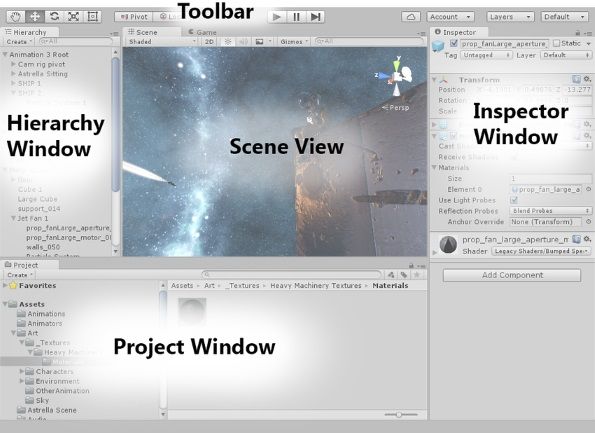
\includegraphics[scale=0.65]{img/InterfaceUnity.jpg}\\
				\vspace{0.5mm}
				\source{\citeonline{unityInterface}}
				\label{fig:interfaceUnity}
			\end{figure}
			
			\begin{table}[ht]
				\caption{Descrição dos painéis na Unity}
				\centering
				\small
				\renewcommand{\arraystretch}{1.2} % Aumenta espaçamento vertical
				\begin{tabular}{m{3.2cm} m{11.8cm}}
					\hline 
					\textit{Project Window} & Exibe a biblioteca de \textit{Assets} que estão disponíveis para uso no projeto. Ao importar os \textit{Assets} no projeto, eles aparecerão aqui. \\ 
					\hline 
					\textit{Scene View} & Permite navegar visualmente e editar a cena. A \textit{Scene View} pode mostrar em perspectiva 3D ou 2D, dependendo do tipo de projeto que está sendo trabalhando. \\ 
					\hline 
					\textit{Hierarchy Window} & É uma representação de texto hierárquica de cada objeto na cena. Cada item na cena tem uma entrada na hierarquia, de forma que as duas janelas estão inerentemente conectadas. A hierarquia revela a estrutura da forma como os objetos estão ligados um ao outro. \\ 
					\hline 
					\textit{Inspector Window} & Permite visualizar e editar todas as propriedades do objeto selecionado. Como diferentes tipos de objetos têm diferentes conjuntos de propriedades, o layout e conteúdo da janela do \textit{Inspector} pode variar. \\ 
					\hline 
					\textit{Toolbar} & Fornece acesso aos recursos de trabalho mais essenciais. À esquerda estão as ferramentas básicas para manipular a \textit{Scene View} e os objetos dentro dela. No centro estão os controles de \textit{play}, \textit{pause} e \textit{step}. Os botões à direita dará acesso aos Serviços da Unity Cloud e da Conta Unity, seguido pelo menu de visibilidade dos \textit{layers} e, finalmente, o menu de \textit{layout} do editor (que fornece alguns \textit{layouts} alternativos para as janelas do editor, e permite salvar um \textit{layout} customizado). \\ 
					\hline 
				\end{tabular}\\
				\vspace{3mm}
				\source{\citeonline{unityInterface}}
				\label{tab:unity}
			\end{table}
			
			Os objetos contidos na cena do projeto são chamados de \textit{GameObject},
			sendo que suas características podem ser alteradas por \textit{Components} anexados a ele.
			A Unity possui vários \textit{Components} prontos,
			no entanto é possível criar novos usando as linguagens de programação do qual se dá suporte (C\# e UnityScript).
			Tais \textit{Components} são chamados de \textit{Scripts},
			e eles permitem disparar eventos,
			modificar as propriedades de outros \textit{Components} ou do próprio \textit{GameObject} durante o jogo,
			e a interação com o jogador.
			\cite{unityScripts}.

	\FloatBarrier
	\section{Visual Studio}
		O Visual Studio é um Ambiente de Desenvolvimento Integrado (IDE) usado para a criação de aplicativos para Windows, Android, iOS, aplicações Web e serviços de nuvem.
		Com ele é possível programar em C\#, Visual Basic, F\#, C++, HTML, JavaScript e Python, dentre outras linguagens de programação. \cite{microsoft}
		
		A integração do Visual Studio com a Unity, usando C\#, ocorre com a adição do \textit{namespace} "\textit{UnityEngine}"{} ao \textit{script},
		%(com o código "using UnityEngine"),
		liberando a utilização da classe \textit{MonoBehaviour},
		da qual possui implementado funcionalidades e funções internas da Unity.
		Para utilizar a classe \textit{MonoBehaviour} nos \textit{scripts} criados,
		basta estender a classe criada com a \textit{MonoBehaviour} \cite{unityScripts}.
		Desta forma, o cabeçalho do \textit{script} fica como no código a seguir:
		
		\begin{lstlisting}[language=C++]
using UnityEngine;

public class NomeDaClasse : MonoBehaviour
{
	// Código da classe
}\end{lstlisting}
		
		Com esta implementação, é possível utilizar uma das principais vantagens do Visual Studio,
		que é o \textit{AutoComplete}.
		Ou seja, funções internas da Unity, como as do \textit{GameObject}, aparecem em uma lista conforme se vai digitando,
		facilitando muito a programação do \textit{script}.
		
		Além da integração com a Unity,
		ainda é possível utilizar as bibliotecas próprias do C\#,
		como bibliotecas matemáticas, acesso à arquivo e listas.
		
		Na Figura \ref{fig:exvs} é possível ver um exemplo de classe criada no Visual Studio que foi usada neste projeto:
		
		\begin{figure}[ht!]
			\caption{Exemplo de classe no Visual Studio}
			\centering
			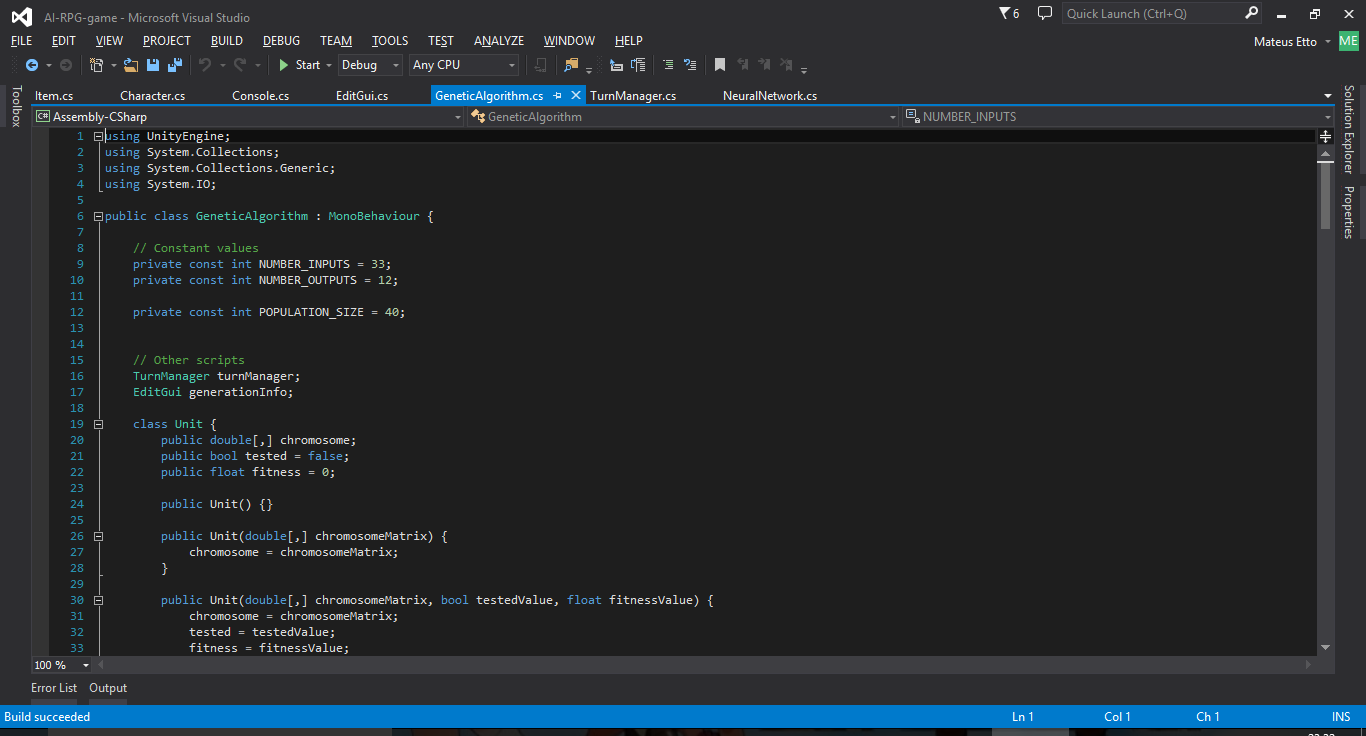
\includegraphics[scale=0.4]{img/InterfaceVisualStudio.png}\\
			\vspace{0.5mm}
			\source{Elaborado pelo autor.}
			\label{fig:exvs}
		\end{figure}
		
		Neste \textit{script} do Algoritmo Genético, além do \textit{UnityEngine} e outras duas bibliotecas básicas do C\#,
		também foi utilizada o \textit{System.IO}, uma biblioteca para Leitura e Escrita de Arquivo.
		Qualquer outro \textit{script} criado para funcionar na Unity tem este padrão.

\FloatBarrier
\newpage % Coloca o conteúdo numa nova página	
\chapter{CONCEITOS}

	Neste capítulo será dada uma introdução sobre o conceito de jogos,
	categorias de jogos que existem,
	e explicado em detalhes sobre o estilo de jogo desenvolvido neste projeto,
	o RPG em turnos.
	Além disto, será descrito dois conceitos que foram amplamente utilizados neste trabalho,
	que são Redes Neurais Artificiais (RNA) e Algoritmo Genético (AG).
	Apesar de ser possível descrever várias variações de aplicação desses conceitos,
	será explicado apenas a essência deles e o que foi necessário para desenvolver este trabalho.
	
	\FloatBarrier
	\section{Jogos}
	% Definição de jogos
	Jogo pode ser definido como uma atividade que provê entretenimento ou diversão{}.
	Nestas seções, jogos serão separados em 2 grandes categorias,
	"jogos não-eletrônicos"{} e "jogos eletrônicos"{}.
	Uma breve descrição e alguns exemplos serão feitos sobre cada um deles.
	
		\FloatBarrier
		\subsection{Jogos não-eletrônicos} \label{ssec:notElectronicGame}
		% Definição de jogos não-eletrônicos
		Jogos não-eletrônicos são os jogos que não requerem um dispositivo eletrônico para ser aproveitado.
		% Breve explicação sobre jogos 'normais' (jogos de criança, como esconde esconde, amarelinha; futebol; jogos de tabuleiro; cartas)
		Brincadeiras como "esconde-esconde"{}, "pega-pega"{} e "amarelinha"{}, por exemplo,
		são jogos comuns entre crianças.
		Futebol e outros esportes também se encaixam nesta categoria.
		% Jogo de mesa
		%No entanto, esta seção irá se focar nos jogos "de mesa"{}.
		
		% Exemplo de jogos de tabuleiro
		Indo para os jogos estratégicos,
		os jogos de tabuleiro são muito comuns.
		Pode-se citar o "xadrez"{} como o mais conhecido de todos,
		com alta complexidade quanto à quantidade de movimentos possíveis e suas consequências.
		Uma variação mais simples é o jogo de "damas"{},
		com menor complexidade e, portanto, mais fácil de aprender.
		Estes jogos são puramente estratégicos,
		sem nenhuma influência da sorte.
		
		% Exemplo de jogos de cartas
		Outros jogos envolvem estratégia e sorte ao mesmo tempo,
		sendo que jogos de cartas podem ser encaixados em tal categoria.
		Jogos muito conhecidos aqui são "\textit{poker}" e "truco",
		do qual os jogadores recebem cartas e fazem estratégias,
		mas dependem da sorte para receber cartas boas.
		
		% Exemplo de jogo RPG (de mesa)
		Por fim, citar-se-á também o jogo RPG de mesa
		(ilustrado na Figura \ref{fig:tableRpg}),
		devido à sua influência nos jogos RPG eletrônicos,
		do qual este trabalho foi inspirado.
		De maneira geral, o RPG de mesa é um jogo do qual cada jogador terá o papel de um personagem em uma história
		(cujo tema é decidido entre os jogadores),
		e um jogador é escolhido como o \textit{Game Master} (GM),
		que irá ditar as consequências da decisão dos jogadores.
		Existem regras a serem seguidas dependendo do jogo que está sendo jogado,
		e dentro destas regras os jogadores são livres para fazerem suas ações.
		É muito comum o áudio dessas partidas serem publicadas na internet,
		por conter histórias interessantes e muitas vezes engraçadas\footnote{Exemplo de áudio de um jogo RPG de mesa: \url{https://jovemnerd.com.br/nerdcast/nerdcast-251-especial-rpg-o-bruxo-a-princesa-e-o-dragao/}}.
		
		% Imagem de pessoas jogando
		\begin{figure}[ht!]
			\caption{Uma partida de RPG de mesa}
			\centering
			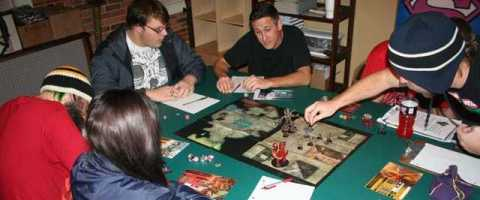
\includegraphics[scale=1.0]{img/RPG_de_mesa.jpg}\\
			\vspace{0.5mm}
			\source{\citeonline{tableRpg}}
			\label{fig:tableRpg}
		\end{figure}
		
		% Introdução ao exemplo prático de Dungeons & Dragons (motivo: relacionado com o trabalho)
		Um exemplo clássico de RPG de mesa é um jogo chamado \textit{Dungeons \& Dragons}.
		% Mecânica do jogo (criação de personagem, atributos, níveis, eventos)
		No início do jogo,
		cada participante escolhe uma "classe"{} e "valores de habilidade",
		anotando-os no "cartão do personagem"{}.
		Após o início da história,
		o \textit{Dungeon Master} (DM), que é equivalente ao GM, conta a história
		e os jogadores escolhem o que querem fazer.
		Ações simples, como abrir uma porta, normalmente resultam em sucesso.
		Mas as consequências de ações mais arriscadas,
		como escapar do ataque de um inimigo,
		são determinadas rolando um dado.
		As probabilidades de sucesso podem mudar dependendo da situação e atributos do personagem.
		Conforme o jogo passa,
		os jogadores ganham pontos de habilidades, experiência e dinheiro.
		%Batalhas contra criaturas místicas acontecem
		%e os jogadores lutam contra elas,
		%determinando o sucesso ou falha dos ataques rolando os dados.
		O jogo continua até o DM encaminhar a história a um final \cite{dungeonsDragons}.
			
	
		\FloatBarrier
		\subsection{Jogos eletrônicos}
		% Definição de jogos eletrônicos
		Jogos eletrônicos são os jogos que usam dispositivos eletrônicos como principal meio para a atividade de entretenimento.
		% Deixar claro que a lista de estilos é maior do que a que está sendo citada aqui
		Existe uma vasta quantidade de estilos de jogos eletrônicos.
		O objetivo desta seção não é mostrar todos,
		mas apenas os principais e mais conhecidos como:
		% Exemplos de estilos de jogos eletrônicos (ação, aventura, role-playing, simulação, esportes, etc)
		ação, aventura, simulação, esportes e RPG.
		
		% Subdivisões de jogos de ação (plataforma, shooter, FPS, luta)
		Mesmo entre jogos de ação,
		existem muitas subdivisões que podem ser feitas,
		e elas inclui-se: plataforma, \textit{shooter} e luta.
		Um exemplo muito conhecido de jogo de plataforma é o \textit{Super Mario World},
		ilustrado na Figura \ref{fig:marioWorld}.
		Jogo \textit{shooter} envolve todos os jogos que há a necessidade de "atirar"{} em inimigos,
		sendo \textit{Space Invaders} um dos primeiros desta categoria a serem criados.
		E jogos de luta, normalmente entre 2 jogadores,
		também fazem parte dos jogos de ação.
		Jogos como \textit{Tekken} e \textit{Mortal Kombat} fazem parte desta categoria \cite{gameGenres}.
		
		\begin{figure}[ht!]
			\caption{Jogo \textit{Super Mario World}}
			\centering
			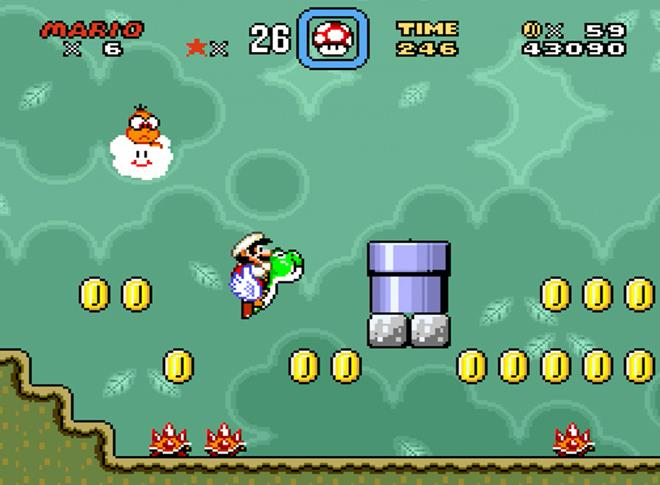
\includegraphics[scale=0.35]{img/marioworld.jpg}\\
			\vspace{0.5mm}
			\source{\citeonline{marioWorld}}
			\label{fig:marioWorld}
		\end{figure}
		
		% Descrição e exemplo de jogos de aventura
		Os jogos de aventura são marcados pela ausência de violência,
		normalmente tendo o seu foco na história.
		Estes jogos se contrastam com os jogos de ação por não precisarem de reflexo por parte do jogador.
		Jogos \textit{point-and-click} se encaixam nesta categoria,
		como o \textit{King's Quest},
		e muitas vezes tem pequenos quebra-cabeças a serem resolvidos \cite{gameGenres}.
		Também existem os \textit{Visual Novels},
		que normalmente possuem gráficos estáticos,
		e o jogador tem escolhas durante a história do jogo,
		alterando o rumo dos acontecimentos.
		Um exemplo pode ser visto na Figura \ref{fig:visualNovel}.
		
		% Imagem de jogo de simulação (F1)
		\begin{figure}[ht!]
			\caption{Exemplo de \textit{Visual Novel}}
			\centering
			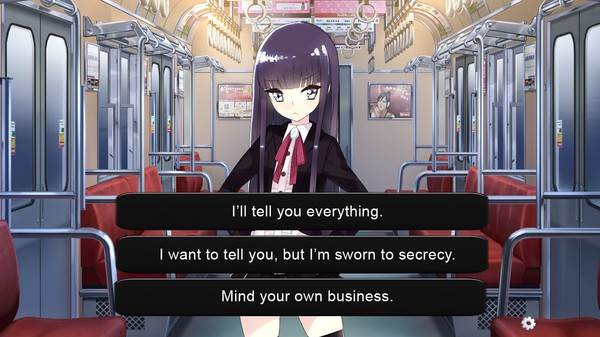
\includegraphics[scale=0.6]{img/visual_novel.jpg}\\
			\vspace{0.5mm}
			\source{\citeonline{visualNovel}}
			\label{fig:visualNovel}
		\end{figure}
		
		% Descrição e exemplo de jogos de simulação
		Os jogos de simulação procuram "imitar"{} a realidade eletronicamente.
		Nestes jogos, um foco muito grande é dado na "cópia"{} das leis da física dentro do jogo,
		permitindo ao jogador um experiência o mais próximo possível da real \cite{gameGenres}.
		Jogos da série Fórmula 1 são um excelente exemplo,
		e pode ser visualizado na figura \ref{fig:formula1}.
		
		\begin{figure}[ht!]
			\caption{Jogo F1 2012}
			\centering
			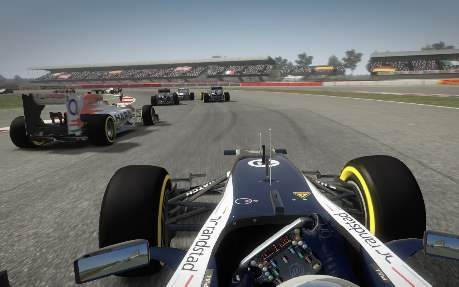
\includegraphics[scale=0.75]{img/formula1.jpg}\\
			\vspace{0.5mm}
			\source{\citeonline{formula1}}
			\label{fig:formula1}
		\end{figure}
		
		% Descrição e exemplo de jogos de esporte
		Jogos de esporte também são populares,
		sendo que as regras são trazidas dos esportes reais \cite{gameGenres}.
		FIFA e \textit{Pro Evolution Soccer} (PES) são exemplos de jogos de futebol muito conhecidos.
		\textit{Mario Tennis} é um exemplo de jogo de tênis usando personagens de \textit{Mario}.
		
		% Descrição e exemplo de jogos RPG
		Por fim, descrever-se-á sobre os jogos RPG,
		que foi o estilo de jogo do qual o projeto deste trabalho se inspirou.
		% Origem dos jogos RPGs eletrônicos
		A origem dos RPGs eletrônicos se dá nos RPGs de mesa,
		%explicado na seção \textit{\ref{ssec:notElectronicGame} Jogos não-eletrônicos},
		com personagens que evoluem com o passar do tempo
		e uma história do qual eles vivem.
		Tais elementos são comuns nas subcategorias de jogos RPG.
		% Explicar a existência de 3 grandes separações possíveis neste estilo de jogo (Ação, Tático e Baseado em Turnos)
		Existem principalmente 3 subcategorias,
		que são: RPG de ação, tático e baseado em turnos.
		A principal diferença entre essas subcategorias está no sistema de batalhas.
		
		% Descrever sobre jogo RPG de Ação
		O RPG de ação utiliza conceitos dos jogos de ação para suas batalhas.
		Ou seja, as batalhas acontecem em tempo real,
		de forma que o pressionar de um botão ativa um golpe ou habilidade.
		Um exemplo é o jogo \textit{Kingdom Hearts},
		ilustrado na Figura \ref{fig:kingdomHearts}.
		A velocidade de reação do jogador é crítica para o resultado da batalha,
		então uma ação efetuada tarde demais pode causar a derrota dele.
		
		% Imagem de RPG de Ação (Kingdom Hearts)
		\begin{figure}[ht!]
			\caption{RPG de ação: \textit{Kingdom Hearts}}
			\centering
			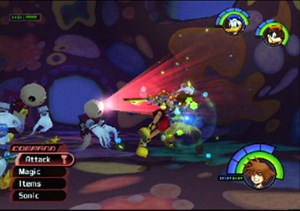
\includegraphics[scale=0.7]{img/kingdom_hearts.jpg}\\
			\vspace{0.5mm}
			\source{\citeonline{wiki_kingdomHearts}}
			\label{fig:kingdomHearts}
		\end{figure}
		
		% Descrever sobre jogo RPG Tático
		Já o RPG tático se assimila mais aos jogos estratégicos, como o xadrez.
		Não existe a liberdade de se mover livremente ou agir rapidamente,
		como no RPG de ação,
		mas de maneira calculada em um mapa que lembra um tabuleiro de xadrez/damas.
		Os personagens tem um padrão ou distância do qual podem se mover,
		assim como distâncias do qual é capaz de realizar ataques.
		\textit{Disgaea} é um exemplo de RPG tático,
		e está ilustrado na Figura \ref{fig:disgaea}.
		
		% Imagem de RPG Tático (Disgaea)
		\begin{figure}[ht!]
			\caption{RPG tático: \textit{Disgaea}}
			\centering
			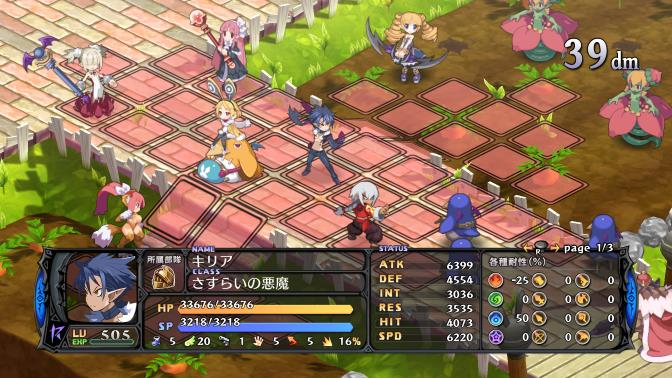
\includegraphics[scale=0.60]{img/disgaea.jpg}\\
			\vspace{0.5mm}
			\source{\citeonline{disgaea}}
			\label{fig:disgaea}
		\end{figure}
		
		% Descrever sobre jogo RPG em Turnos
		O RPG em turnos difere dos demais pela não necessidade de posicionar os personagens para efetuar os comandos.
		Um exemplo é \textit{Mana Khemia}, ilustrado na Figura \ref{fig:manaKhemia}.
		Os personagens recebem turnos de forma sistemática
		(um de cada vez)
		ou dependente de um atributo,
		 como a "velocidade".
		Ao receber o turno, o jogador decide qual será o melhor comando a ser atribuído ao personagem,
		com o objetivo de vencer a batalha.
		
		% Imagem de RPG em Turnos (Mana Khemia)
		\begin{figure}[ht!]
			\caption{RPG em turnos: \textit{Mana Khemia}}
			\centering
			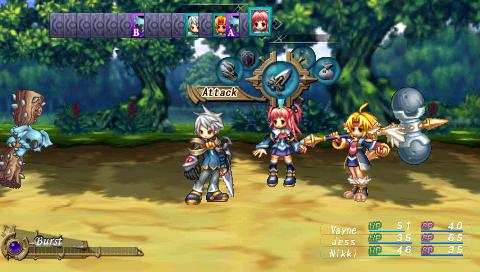
\includegraphics[scale=0.55]{img/mana-khemia.jpg}\\
			\vspace{0.5mm}
			\source{\citeonline{manaKhemia}}
			\label{fig:manaKhemia}
		\end{figure}
		
		% Relembrar que podem existir variações dentro destas definições
		Por fim, vale lembrar que apesar de existirem essas separações por categorias dos jogos,
		muitas vezes os jogos são híbridos,
		então eles podem conter características de várias categorias ao mesmo tempo.
		% O escolhido neste trabalho foi o jogo RPG em Turnos
		A categoria que foi escolhida para desenvolver o projeto deste trabalho foi o RPG em turnos,
		então muitas de suas características estão presentes no jogo desenvolvido neste projeto.
		

	\FloatBarrier
	\section{Redes Neurais Artificiais}
	% 1 Definição
	As RNAs são uma família de modelos inspirados no funcionamento do cérebro humano,
	sendo que a "baixo nível"{} procuram imitar o que acontece nos neurônios.
	São usadas para estimar ou aproximar funções que dependam de um grande número de entradas. \cite{bookAI-ANNdefinition}
	
	\subsection{Funcionamento}
	% 2 Arquitetura
	% 2.1 Funções de entrada e ativação
	A unidade em uma RNA é o neurônio.
	O neurônio recebe estímulos, que na RNA são números reais.
	Recebendo os vários estímulos, o neurônio faz uma operação com todos os números recebidos,
	que normalmente é um somatório.
	Esta é a função de entrada.
	
	Após aplicar a função de entrada em todos os estímulos,
	é obtido um único valor.
	Este valor, então, é processado por uma função de ativação.
	Existem várias funções de ativação que podem ser utilizadas,
	e pode-se ver alguns exemplos na Figura \ref{fig:activationFunctions}.
	
	\begin{figure}[ht!]
		\caption{Funções de Ativação comuns em uma RNA}
		\centering
		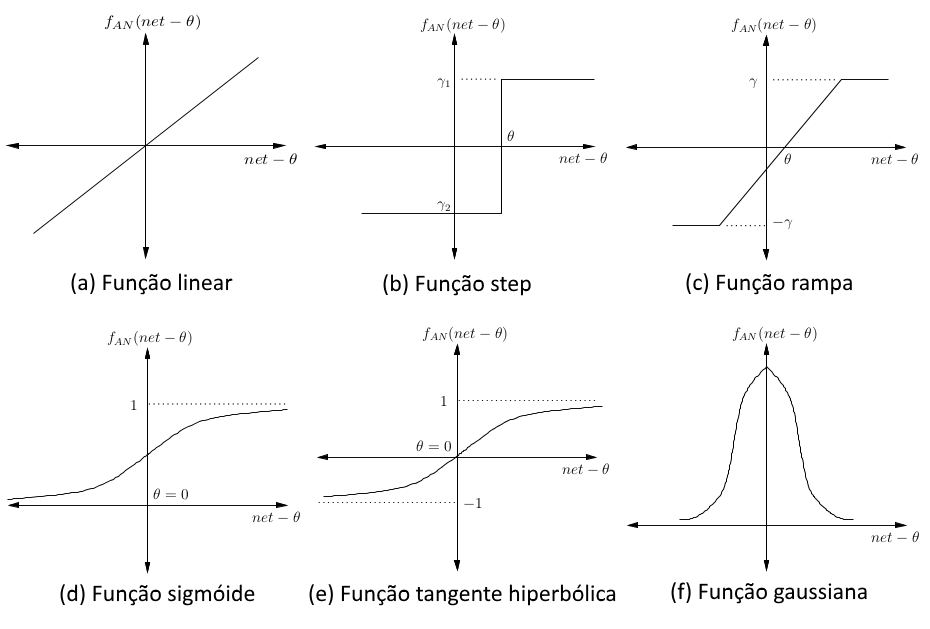
\includegraphics[scale=0.48]{img/ActivationFunctions.png}\\
		\vspace{0.5mm}
		\source{Baseado em \citeonline{turingFinance}}
		\label{fig:activationFunctions}
	\end{figure}
	
	Diferentes funções de ativação se adequam melhor dependendo da aplicação da RNA,
	assim como a camada em que o neurônio se encontra.
	
	O resultado da função de ativação é então multiplicado por um peso,
	e passado para o próximo neurônio como um estímulo. \cite{bookAI-ANNdefinition}
	
	% 2.2 Particularidades (camadas existentes, papel de cada uma)
	A arquitetura de uma RNA é formada por uma camada de entrada (\textit{input layer}),
	uma camada de saída (\textit{output layer}),
	e as camadas ocultas (\textit{hidden layers})
	que poderão conter de zero a muitas camadas.
	Cada camada na RNA terá \textit{n} neurônios,
	sendo \textit{n} qualquer valor maior ou igual a 1.
	Um exemplo de RNA com uma camada oculta pode ser visto na Figura \ref{fig:basicnn}.
	
	\begin{figure}[ht!]
		\caption{RNA com uma camada oculta}
		\centering
		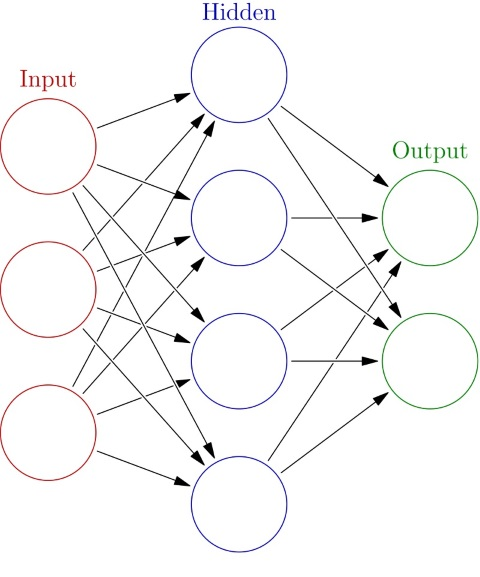
\includegraphics[scale=0.45]{img/BasicNN.jpg}\\
		\vspace{0.5mm}
		\source{\citeonline{wikimedia}}
		\label{fig:basicnn}
	\end{figure}
	
	Como ilustrado na Figura \ref{fig:basicnn},
	cada neurônio de uma camada se conecta com todos os outros neurônios da camada seguinte.
	Existem muitas variações de arquiteturas de RNA,
	não sendo todas que seguem o padrão visto na Figura \ref{fig:basicnn},
	porém esta é a arquitetura mais "tradicional"{}.
	
	Uma RNA sempre terá uma camada de entrada e uma de saída.
	No entanto, o número de camadas ocultas pode variar bastante entre um problema e outro.
	Estas camadas ocultas são explicadas como sendo "extratoras de características"{}
	\cite{stackExchange2}.
	
	Então, se o número de camadas ocultas varia,
	de que maneira pode-se determinar o número de camadas ocultas a serem utilizadas em um determinado problema?
	Caso os dados sejam linearmente separáveis,
	não é necessário nenhuma camada oculta.
	Por outro lado, se forem dados não lineares,
	uma ou mais camadas ocultas serão necessárias
	\cite{stackExchange1}.
	
	Quanto mais camadas ocultas forem utilizadas,
	maior a granularidade dos resultados obtidos na RNA,
	como pode ser visto na Figura \ref{fig:nnhiddenlayer}.
	Para garantir esta não-linearidade dos resultados, %ao utilizar mais de uma camada oculta na RNA,
	é necessário colocar funções de ativação não-lineares nos neurônios das camadas ocultas.
	
	\begin{figure}[ht!]
		\caption{Importância da camada oculta}
		\centering
		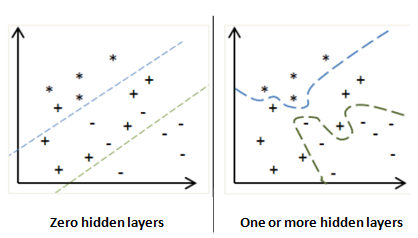
\includegraphics[scale=1.5]{img/HiddenLayers.png}\\
		\vspace{0.5mm}
		\source{\citeonline{stackOverflow1}}
		\label{fig:nnhiddenlayer}
	\end{figure}
	
	Deve-se lembrar que, apesar de muitas camadas ocultas aumentar a granularidade dos resultados,
	isto vem com um custo:
	mais tempo de processamento e
	aprendizagem mais lenta.
	É por este motivo que deve-se buscar a arquitetura (número de camadas ocultas e número de neurônios) otimizada ao problema,
	com baixo tempo de processamento e alto desempenho.
	
	Existem muitas discussões a respeito do número otimizado de camadas ocultas a serem usadas, caso ela seja necessária.
	Um consenso que existe é que uma única camada é o suficiente para a maioria dos problemas
	\cite{stackExchange1}.
	
	Considerando a necessidade de colocar uma camada oculta na RNA,
	existem regras empíricas que ajudam a escolher um número de neurônios a serem colocados na camada oculta.
	Uma delas é encontrar a média do número de neurônios de entrada e de saída,
	e usar este valor como ponto de partida,
	ajustando-o então com testes
	\cite{stackExchange1}.
	
	\subsection{Tipos de aprendizado}
	% 3 Tipos de aprendizado (com exemplos de utilização)
	Um dos maiores atrativos de uma RNA é sua capacidade de aprender,
	e atualmente existem três paradigmas de aprendizagem:
	Aprendizado Supervisionado, Aprendizado Não-supervisionado e Aprendizado Reforçado.
	
	No Aprendizado Supervisionado,
	tem-se os dados de entrada, e infere-se os dados de saída.
	Sabendo-se estas duas informações, treina-se a RNA para que produza os resultados esperados,
	ajustando os pesos de suas conexões.
	Esta forma de aprendizagem é utilizada principalmente para duas finalidades:
	reconhecimento de padrões e regressão de funções.
	
	Dependendo da finalidade da RNA no Aprendizado Supervisionado,
	diferentes funções de ativação são recomendadas na camada de saída
	(as funções de ativação podem ser vistas na Figura \ref{fig:activationFunctions}, página \pageref{fig:activationFunctions}).
	Caso a tarefa da RNA seja de reconhecer padrões,
	as funções recomendadas são a \textit{step} (b), sigmoide (d) e tangente hiperbólica (e).
	Por outro lado, se a tarefa for de regressão de uma função,
	a função linear (a) é a mais recomendada \cite{researchGate}.
	
	No Aprendizado Não-supervisionado,
	tem-se os dados de entrada e uma função de custo a ser minimizada.
	Com o decorrer das iterações,
	os pesos da RNA serão adaptados para minimizar o custo.
	Tarefas que usam tal paradigma são os que envolvem problemas de estimativa.
	
	No Aprendizado Reforçado,
	os dados de entrada são desconhecidos,
	e o cálculo do custo é feita de maneira dinâmica.
	Os dados de entrada são gerados através das interações do RNA com o ambiente.
	Exemplos de utilização deste paradigma são
	programação dinâmica e problemas de controle.

	\FloatBarrier
	\section{Algoritmo Genético}
	% 1 Definição
	Algoritmo Genético (AG) faz parte da computação evolutiva,
	e inspirou-se na teoria de Darwin sobre a evolução das espécies.
	É uma busca heurística usada para encontrar soluções de otimização e resolver problemas de busca. \cite{obitko}
	
	\FloatBarrier
	\subsection{Conceitos de AG}
	% 2 Conceitos
	% 2.1 Cromossomos
	A unidade que caracteriza um determinado indivíduo na população é o cromossomo.
	% 2.1.1 Gene
	O cromossomo é constituído de vários genes,
	que carregam informações ou características de um indivíduo. %que carregam informação ou característica de um indivíduo.
	% 2.1.2 Representação do cromossomo
	O gene pode ser representado de várias formas dentro do AG,
	sendo a mais simples delas a representação binária,
	como pode ser visto na Tabela \ref{tab:cromosome}.
	
	\begin{table}[ht]
		\caption{Representação binária de cromossomos}
		\centering
		\begin{tabular}{c c c c c c c c c c c}
			\hline 
			0 & 1 & 1 & 0 & 1 & 0 & 0 & 0 & 1 & 0 & 1\\ 
			\hline 
			1 & 0 & 1 & 0 & 0 & 1 & 1 & 0 & 0 & 1 & 0\\ 
			\hline 
		\end{tabular} \\
		\vspace{3mm}
		\source{Elaborado pelo autor.}
		\label{tab:cromosome}
	\end{table}
	
	Outras representações de cromossomos também existem.
	Por exemplo, existe a codificação por permutação,
	utilizado em problemas de ordenação.
	Neste caso, todo cromossomo é um vetor de números,
	e cada número representa uma posição.
	
	Outro exemplo é codificação por valor.
	Este valor poderá ser qualquer coisa relacionada ao problema,
	como números reais ou sequência de caracteres.
	E como último exemplo existe a codificação em árvore,
	em que cada cromossomo é uma árvore de objetos,
	como funções ou comandos em uma linguagem de programação.
	
	% 2.2 Indivíduo
	Um indivíduo no AG sempre possuirá um cromossomo.
	Este indivíduo carrega uma das possíveis soluções do problema.
	%e pode ser uma solução boa ou não.
	
	% 2.3 População
	O indivíduo faz parte de uma população.
	%Logo, pode-se dizer que uma população é um conjunto de soluções.
	% 2.3.1 Tamanho de população
	Para se resolver um problema usando AG,
	nem sempre uma população enorme irá se traduzir em uma convergência mais rápida.
	De acordo com algumas pesquisas,
	população em torno de 30 indivíduos se mostram ser eficientes,
	apesar de que outros valores possam ser melhores dependendo do problema
	\cite{obitko}.
	
	% 2.4 Geração
	Uma geração diz respeito à iteração do qual a população se encontra.
	Uma população nova criada a partir de uma população antiga é uma nova geração.
	Tem-se, então, várias gerações de populações diferentes (ou evoluídas).
	
	% 2.5 Avaliação
	% 2.5.1 Fitness (aptidão)
	Durante o algoritmo do AG, deve-se calcular o o \textit{fitness} (nível de aptidão) de cada indivíduo da população.
	A forma de se calcular o \textit{fitness} do indivíduo depende do problema,
	e este cálculo faz parte do processo de Avaliação da população,
	que pode ser visto em mais detalhes na Tabela \ref{tab:agCycle} e Figura \ref{fig:gaflow},
	na seção \ref{ssec:processo}.
	
	% 2.6 Seleção
	No processo de Seleção,
	indivíduos da população são selecionados para passarem para a próxima geração ou se reproduzirem.
	A Seleção usa o valor de \textit{fitness} para dar maiores chances de selecionar os indivíduos mais adaptados.
	
	% 2.6.1 Roleta
	Um método comum para se selecionar indivíduos é o método da Roleta.
	Neste método, um intervalo numérico relativo ao valor de \textit{fitness} é atribuído a cada indivíduo.
	Então é sorteado aleatoriamente um valor no intervalo de todos os indivíduos.
	O indivíduo que conter o número sorteado dentro de seu intervalo é o escolhido para passar para a próxima geração ou se reproduzir.
	Percebe-se assim que indivíduos com maior \textit{fitness} terão um intervalo maior e, portanto, maiores chances de serem selecionados.
	Uma ilustração do que foi descrito pode ser visto na Figura \ref{fig:roulette}.
	
	\begin{figure}[ht!]
		\centering
		\caption{Método da roleta para Seleção}
		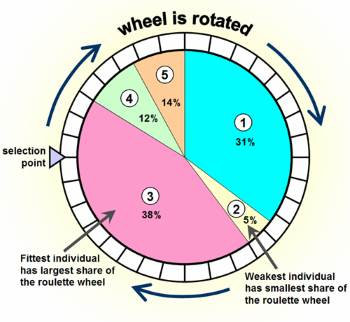
\includegraphics[scale=0.8]{img/Roulette.jpg}\\
		\vspace{0.5mm}
		\source{\citeonline{stackOverflow2}}
		\label{fig:roulette}
	\end{figure}
	
	% 2.6.2 Ranking
	Outro exemplo de método de Seleção é o de \textit{Ranking}.
	De forma similar ao da Roleta, é usado o valor de \textit{fitness}.
	No entanto, o diferencial está no fato de ordenar os indivíduos em um \textit{ranking},
	e atribuir um intervalo numérico dependendo do \textit{ranking} do indivíduo
	(quanto maior o \textit{ranking}, maior o intervalo atribuído).
	
	% 2.7 Crossover
	Após a seleção existe o \textit{Crossover} (ou cruzamento).
	%análogo à reprodução que se estuda em biologia.
	Se for decidido que haverá um \textit{crossover},
	informações do cromossomo de 2 indivíduos serão misturados,
	criando "cromossomos filhos"{}.
	Neste processo, são selecionados pontos nos cromossomos pais,
	e os cromossomos filhos copiam do primeiro cromossomo pai até aquele ponto,
	passando então a copiar do segundo cromossomo pai.
	O \textit{crossover} pode ter um único ponto ou vários pontos de \textit{crossover}.
	Também existe o \textit{crossover} uniforme,
	em que é copiado vários pequenos trechos de ambos os pais,
	com taxa de 50\%.
	
	% 2.7.1 Taxa de Crossover
	No entanto, o \textit{crossover} não necessariamente ocorre.
	Existe uma probabilidade dele acontecer,
	e essa probabilidade é a taxa de \textit{crossover}.
	Considerando-se, por exemplo, uma taxa de \textit{crossover} de 90\%,
	tem-se que 90\% dos indivíduos selecionados passarão pelo processo de \textit{crossover},
	e que 10\% serão copiados para a nova população.
	
	% 2.8 Mutação
	Após o \textit{crossover},
	os cromossomos passam pelo processo de Mutação.
	A mutação permite a mudança de alguns genes escolhidos aleatoriamente.
	% 2.8.1 Taxa de Mutação
	A chance de ocorrer uma mutação em um determinado gene é determinado pela taxa de mutação.
	Por exemplo, se a taxa de mutação for de 1\%,
	isto significa que 1\% dos genes terão seus valores alterados.
	
	% 2.9 Elitismo
	A fim de não se perder boas soluções por causa do \textit{Crossover} e Mutação,
	uma técnica muito aplicada e eficiente é a do Elitismo.
	Nesta técnica, o melhor (ou melhores) indivíduos da população são copiados sem nenhuma alteração para a próxima geração.
	
	\FloatBarrier
	\subsection{Processo} \label{ssec:processo}
	% 3 Processo
	O AG mais simples de ser representado tem 5 etapas,
	em um processo que se repete até que uma determinada condição de parada seja satisfeita.
	O processo ocorre como explicado na Tabela \ref{tab:agCycle} e ilustrado na Figura \ref{fig:gaflow}.
	
	\begin{table}[h]
		\caption{Ciclo do Algoritmo Genético}
		\centering
		\small
		\renewcommand{\arraystretch}{1.2} % Aumenta espaçamento vertical
		\begin{tabular}{>{\centering\arraybackslash}m{3.5cm} m{11.5cm}}
			\hline 
			\textbf{Inicia População} & Gera uma população aleatória de n indivíduos. \\ 
			\hline 
			\textbf{Avaliação} & Calcula o valor de \textit{fitness} de cada cromossomo na população. Se a condição de parada for satisfeita, o algoritmo acaba. \\ 
			\hline 
			\textbf{Seleção} & Seleciona 2 cromossomos de acordo com o \textit{fitness}. Quanto maior o valor de \textit{fitness}, maior a probabilidade de ser selecionado. \\ 
			\hline 
			\textbf{\textit{Crossover}} & Copia partes dos cromossomos dos pais em cromossomos filhos, inserindo-os na nova população. \\ 
			\hline 
			\textbf{Mutação} & Aplica a probabilidade de alterar aleatoriamente os genes dos indivíduos da nova população, e retorna ao passo de Avaliação. \\ 
			\hline 
		\end{tabular}\\
		\vspace{3mm}
		\source{Elaborado pelo autor.}
		\label{tab:agCycle}
	\end{table}
	
	\begin{figure}[ht!]
		\centering
		\caption{Passo a passo do AG}
		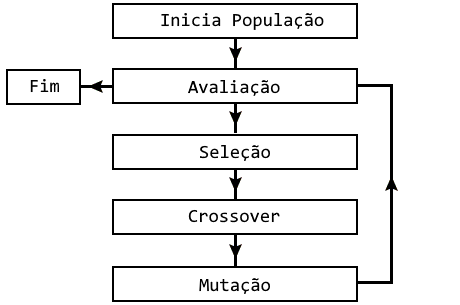
\includegraphics[scale=0.7]{img/GeneticAlgorithmFlow.png}\\
		\vspace{0.5mm}
		\source{Baseado em \citeonline{techEffigy}}
		\label{fig:gaflow}
	\end{figure}
	
	A condição de parada pode ocorrer por mais de um motivo.
	A melhor condição para se parar é uma boa "avaliação"{} (\textit{fitness}) dos indivíduos,
	mas também é possível parar por causa de um limite de gerações ou iterações.
	
	Como é possível notar,
	a repetição das etapas de Avaliação, Seleção, \textit{Crossover} e Mutação melhora gradativamente as soluções encontradas,
	sendo esta a maior motivação de se utilizar um AG.	
	
	\FloatBarrier
	\subsection{Exemplos de aplicação}
	% 4 Exemplos de aplicação
	Como exemplos de aplicação de AG,
	será citado
	Design Automotivo, Robótica, Otimização de rotas e Jogos.
	
	No caso de Design Automotivo,
	AGs podem auxiliar na escolha de materiais e seus formatos para a produção de veículos mais rápidos, leves, econômicos e mais seguros.
	A Figura \ref{fig:automotiveDesign} ilustra um exemplo de design de carro.
	Por se tratar de um problema de otimização,
	o AG pode encontrar várias soluções que irão ajudar o \textit{designer} a projetar o veículo
	\cite{brainz}.
	
	\begin{figure}[ht!]
		\centering
		\caption{Exemplo de \textit{design} de carro}
		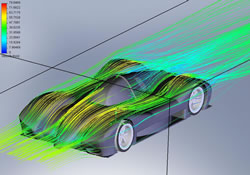
\includegraphics[scale=0.7]{img/AutomotiveDesign.jpg}\\
		\vspace{0.5mm}
		\source{\citeonline{brainz}}
		\label{fig:automotiveDesign}
	\end{figure}
	
	A aplicação de AG em Robótica procura os \textit{designs} de robôs mais otimizados para as suas tarefas.
	Como existem muitas "tarefas"{} que podem ser dadas aos robôs,
	diferentes \textit{designs} são necessários.
	Um AG pode agilizar o processo de desenvolvimento de \textit{design} de um robô,
	considerando as inúmeras variáveis e criando um \textit{design} melhorado
	\cite{brainz}.
	
	AGs também são capazes de encontrar boas soluções em problemas de otimização de rotas.
	As rotas podem ser de, por exemplo:
	um navio no oceano,
	um carro na estrada ou cidade,
	e dados trafegando por roteadores na internet
	\cite{brainz}.
	
	Como último exemplo,
	é possível utilizar AG em jogos eletrônicos.
	O jogo The Sims permite que o jogador crie uma família e treine-a para se relacionar uns com os outros
	\cite{brainz}.
	O jogo Creatures simula a vida pequenas criaturas,
	e procura ser fiel ao simular a vida deles como se fossem pequenos animais,
	criando seu "DNA"{} e características passadas geneticamente
	\cite{aigamedev}.
	
	\FloatBarrier
	\subsection{Variação com RNA}
	Uma diferente forma de se trabalhar com AG é juntá-la com RNA.
	Desta maneira, a RNA terá como papel o processamento de dados complexos,
	e o AG fará a busca dos pesos otimizados na RNA.
	
	Na Figura \ref{fig:nn-ag}, é possível visualizar como é implementação dos conceitos juntos.
	
	\begin{figure}[ht!]
		\centering
		\caption{RNA e AG juntos}
		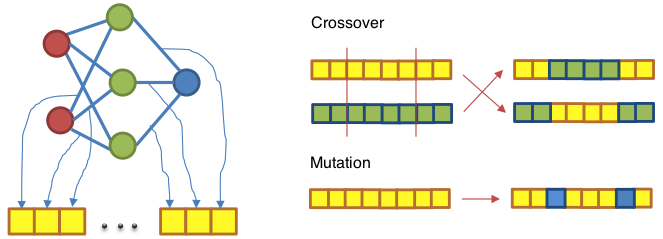
\includegraphics[scale=0.7]{img/NeuralNetworkIntoChromosome.png}\\
		\vspace{0.5mm}
		\source{\citeonline{evoNNAgents}}
		\label{fig:nn-ag}
	\end{figure}
	
	Os pesos da RNA são colocados na estrutura do cromossomo,
	e então é tratado como um cromossomo para realizar o processo do AG.
	Ao finalizar, o cromossomo retorna à RNA como pesos,
	usa-se e repete o processo.
	
	Este foi o método escolhido para a criação da aplicação de Inteligência Artificial neste trabalho:
	Algoritmo Genético otimizando os pesos de uma Rede Neural Artificial.

\FloatBarrier
\newpage % Coloca o conteúdo numa nova página
\chapter{O JOGO}

	Este capítulo descreverá como foi desenvolvido o jogo,
	fórmulas criadas e todos os detalhes relevantes para o entendimento do funcionamento do jogo e de sua aplicação de Inteligência Artificial.
	
	\FloatBarrier
	\section{Descrição do jogo}
	% 1 Visão geral do jogo
	O jogo desenvolvido neste projeto é um jogo RPG em turnos,
	do qual 2 times de 3 personagens cada se enfrentam numa batalha cujo objetivo é derrotar o time inimigo.
	
	% 2 Descrição breve de como ocorre a batalha (turnos, 3x3, colocar imagem)
	A complexidade do jogo se compõe de:
	uma lista de atributos para cada personagem,
	diferentes habilidades para dar dano ou curar,
	e itens consumíveis,
	tudo junto com uma verificação elemental que pode dar alguma vantagem ao dano ou não.
	A seguir será descrito cada uma destas partes.
	
	% 3 Explicar detalhadamente cada atributo de personagem
	% 3.1 Atributos (em que favorecem, desfavorecem ou melhoram durante a batalha)
	\subsection{Descrição dos atributos}
	%Primeiramente será explicado a respeito dos atributos de cada personagem,
	%e está descrito na Tabela \ref{tab:characterStats}.
	A Tabela \ref{tab:characterStats} a seguir define quais são os atributos dos personagens,
	e mostra uma breve descrição de seu papel durante o jogo.
	
	\begin{table}[h]
		\caption{Atributos dos personagens}
		\centering
		\small
		\renewcommand{\arraystretch}{1.2} % Aumenta espaçamento vertical
		\begin{tabular}{>{\centering\arraybackslash}m{3.5cm} m{11.5cm}}
			\hline 
			\textbf{HP (\textit{Health Points})} & Pontos de vida, é o quanto de dano o personagem pode receber antes de ser incapacitado. \\ 
			\hline 
			\textbf{MP (\textit{Magic Point}s)} & Pontos de magia, é consumido ao utilizar habilidades. \\ 
			\hline 
			\textbf{ATK (\textit{Attack})} & Um valor alto de ataque permite infligir maiores danos físicos. \\ 
			\hline 
			\textbf{DEF (\textit{Defense})} & Um valor alto de defesa reduz os danos físicos que serão infligidos no HP. \\ 
			\hline 
			\textbf{MAG (\textit{Magic})} & Equivalente ao ATK, mas infligindo danos mágicos. \\ 
			\hline 
			\textbf{RES (\textit{Resistance})} & Equivalente ao DEF, mas reduzindo danos mágicos que serão infligidos no HP. \\ 
			\hline 
			\textbf{SPD (\textit{Speed})} & Velocidade do personagem, e valores altos o permite executar mais comandos em menos tempo. \\ 
			\hline 
		\end{tabular}\\
		\vspace{3mm}
		\source{Elaborado pelo autor.}
		\label{tab:characterStats}
	\end{table}
	
	Percebe-se que existe uma diferenciação de 2 tipos básicos de danos:
	o físico e o mágico.
	%Desta forma, no momento do ataque é verificado qual é o tipo de dano a ser causado.
	Para ambos os casos
	existem atributos ofensivos que tendem a aumentar o dano (ATK para dano físico e MAG para dano mágico),
	e atributos defensivos que tendem a reduzir o dano (DEF para dano físico e RES para dano mágico).
	
	Após um calculo de dano,
	aquele valor é subtraído no HP do defensor.
	Caso o HP deste personagem chegue a 0,
	ele é considerado como incapacitado e não participa mais da batalha.
	
	A única maneira de causar danos mágicos é através de habilidades.
	Como visto na Tabela \ref{tab:characterStats},
	utilizá-las consome MP.
	Caso o MP seja insuficiente para utilizar a habilidade,
	ela não poderá ser usada.
	
	% 3.2 Explicar sobre as fraquezas e pontos fortes, elementos e suas taxas no dano
	Assim como os personagens tem atributos,
	eles também tem uma lista de pontos fracos e fortes.
	Esta lista é composta por 5 diferentes danos que é possível receber
	(sendo 4 delas sub-divisões do dano mágico)
	e seu valor (alta resistência, normal ou fraco).
	Mais detalhes sobre tipos de danos podem ser vistos na Tabela \ref{tab:damageTypes}.
	
	\begin{table}[h]
		\caption{Tipos de danos}
		\centering
		\small
		\renewcommand{\arraystretch}{1.2} % Aumenta espaçamento vertical
		\begin{tabular}{>{\centering\arraybackslash}c|c}
			%\hline 
			%\textbf{Tipo de dano} & \textbf{Sub-divisão} \\ 
			\hline 
			Ataque físico & Dano físico \\ 
			\hline 
			\multirow{4}{*}{Ataque mágico (elemental)}	& Dano de água \\\cline{2-2}
														& Dano de fogo \\\cline{2-2}
														& Dano de terra \\\cline{2-2}
														& Dano de vento \\
			\hline 
		\end{tabular}\\
		\vspace{3mm}
		\source{Elaborado pelo autor.}
		\label{tab:damageTypes}
	\end{table}
	
	Então se um determinado personagem tiver fraqueza em dano de água e levar este tipo de ataque,
	o dano a ser causado em seu HP será aumentado em relação ao dano normal.
	Por outro lado, se este mesmo personagem for resistente à água,
	o mesmo ataque teria o dano no HP reduzido em relação ao dano normal.
	
	% 3.3 Cálculo do dano, skills existentes, suas taxas de dano, elemento e consumo de MP
	\subsection{Cálculos de dano e velocidade}
	%O primeiro passo para o cálculo de um dano neste jogo é o cálculo de um multiplicador,
	%que é calculado da seguinte forma:
	
	%\begin{equation}
	%	Multiplicador = \begin{cases}
	%				\frac{ATK}{0,3 ATK + 1,2 DEF}	& se \frac{ATK}{0,3 ATK + 1,2 DEF} \geq 0,2 \\
	%					0,2								& se \frac{ATK}{0,3 ATK + 1,2 DEF} < 0,2
	%					\end{cases}
	%	\label{eq:multiplier}
	%\end{equation}
	As fórmulas que aparecem nesta seção foram criadas de forma empírica,
	e foram frequentemente testadas no jogo a fim de deixá-lo equilibrado.
	
	O cálculo de danos no jogo é realizado pelas seguintes fórmulas:
	
	\begin{equation}
		\textrm{Dano} = 0,3 \textrm{ ATK} \times \left(\frac{\textrm{ATK}}{0,3 \textrm{ ATK} + 1,2 \textrm{ DEF}}\right)
		\label{eq:physicalDamageFormula}
	\end{equation}
	
	\begin{equation}
		\textrm{Dano} = 0,3 \textrm{ MAG} \times \left(\frac{\textrm{ MAG}}{0,3 \textrm{ MAG} + 1,2 \textrm{ RES}}\right)
		\label{eq:magicalDamageFormula}
	\end{equation}
	
	\vspace{3mm}
	
	A fórmula \eqref{eq:physicalDamageFormula} é usada para calcular danos físicos,
	e o valor de ATK a ser usado é do atacante,
	DEF é do defensor,
	e o dano calculado é o que será reduzido do HP do defensor.
	
	A fórmula \eqref{eq:magicalDamageFormula} é usada para calcular danos mágicos,
	sendo MAG atributo do atacante,
	RES do defensor,
	e como a primeira fórmula, o dano é subtraído do HP do defensor.
	
	Após o cálculo do dano,
	é verificado qual é o tipo de dano a ser atribuído
	(detalhes dos tipos de danos estão na Tabela \ref{tab:damageTypes}),
	e qual a resistência àquele tipo de dano em específico que o defensor tem.
	Caso o defensor tenha fraqueza neste tipo de ataque,
	o dano ainda passa pela Fórmula \eqref{eq:damageBonus}.
	
	\begin{equation}
		\textrm{Dano final} = 1,5 \times \textrm{dano}
		\label{eq:damageBonus}
	\end{equation}
	
	\vspace{3mm}
	
	Por outro lado, caso o defensor tenha resistência no tipo do dano,
	a fórmula a ser usada será a Fórmula \eqref{eq:damageReduction}
	
	\begin{equation}
		\textrm{Dano final} = 0,6 \times \textrm{dano}
		\label{eq:damageReduction}
	\end{equation}
	
	\vspace{3mm}
	
	Se o personagem não tem fraqueza nem resistência ao dano,
	o dano final será o mesmo que o calculado nas Fórmulas \eqref{eq:physicalDamageFormula} e \eqref{eq:magicalDamageFormula}.
	
	Por último, tem-se a influência do SPD na frequência de se efetuar comandos.
	A partida é composta por vários turnos,
	e é possível que ninguém ou apenas um personagem efetue alguma ação.
	Os personagens tem uma variável de "preparado para efetuar comando"{} que inicia-se em 0 e completa-se ao chegar em 1000
	(mas não se limitando a este valor).
	Em todos os turnos, todos os personagens ganham pontos nessa variável,
	e a quantidade que ganham é determinada pela Fórmula \eqref{eq:speedCalculation} a seguir:
	
	\begin{equation}
		\textrm{Preparado} = \textrm{Preparado} + \textrm{SPD}
		\label{eq:speedCalculation}
	\end{equation}
	
	\vspace{3mm}
	
	Após este cálculo,
	o jogo ordena todos os personagens que ainda estão batalhando de acordo com esta variável.
	Se o primeiro da lista tiver 1000 pontos ou mais, um turno é atribuído a ele,
	a variável dele é reduzida em 1000 pontos,
	voltando assim ao final da lista.
	
	As fórmulas aqui apresentadas foram usadas na implementação do jogo,
	mas é importante deixar claro que também foi adicionado aleatoriedade nas fórmulas,
	a fim de aumentar a complexidade do jogo e deixá-lo menos determinístico.
	Os danos finais podem variar 15\% para mais ou para menos do que foi calculado.
	E a velocidade, no cálculo do "preparado"{}, SPD tem um acréscimo aleatório entre 0 e 9 unidades.
	
	% 4 Comandos: Ataque, Defesa, Skill (3.3) e Item - Explicar cálculos executados
	\subsection{Comandos}
	Quando um personagem recebe um turno,
	ele pode escolher um entre 4 comandos básicos:
	Atacar, Defender, Usar Habilidade e Usar Item.
	
	\textbf{Ataque} é o comando ofensivo mais simples de todos.
	Não consome MP,
	e causa dano físico razoavelmente baixo.
	
	\textbf{Defesa} é um comando defensivo que reduz o dano a ser recebido.
	Após todos os cálculos de dano,
	é verificado se o personagem está defendendo.
	Se estiver, aquele dano é reduzido em 50\%.
	
	\textbf{Habilidade} é um comando que possui 3 subcomandos,
	cada um deles representando uma habilidade diferente:
	
	\begin{itemize}[noitemsep]
    	\item \textbf{Habilidade Fraca} é uma habilidade que pode causar tanto dano físico quanto mágico,
		consome 50 MP,
		e após os cálculos de dano,
		o valor de dano é aumentado em 50\%.
    	\item \textbf{Habilidade Forte} é semelhante a fraca,
    	consome 110 MP,
		e causa um aumento de dano de 100\%.
    	\item \textbf{Habilidade de Cura} é uma habilidade que permite recuperar o HP de algum personagem.
		Por ser uma habilidade de suporte,
		a RES do alvo é ignorada,
		sendo aplicada uma cura equivalente a 50\% do MAG do personagem que está aplicando a cura.
  	\end{itemize}
	
	\textbf{Item} é um comando que permite o uso de itens consumíveis durante a batalha.
	Existem 6 itens diferentes,
	um é Poção e os outros 5 são ofensivos, um para cada tipo de dano existente no jogo.
	A poção tem valor constante de cura,
	e os outros tem um valor de "ataque"{} semelhante a ATK ou MAG,
	que é independente do personagem que irá usá-lo.
	
	% 5 Times: Valores atribuídos para cada personagem (stats, fraq. e ponto forte, elem. das skills)
	\subsection{Atributos dos personagens}
	A escolha dos valores de atributos,
	elemento das habilidades,
	pontos fracos e fortes foram definidos de forma a deixar a batalha estratégica e interessante.

	Os personagens de ambos os times foram criados com parâmetros iguais,
	de forma que se tenha uma batalha de "igual para igual"{}.
	Todas estas informações foram resumidas
	e estão ilustradas na Tabela \ref{tab:charactersParamters}.
	
	\begin{table}[h]
		\caption{Parâmetro dos personagens}
		\centering
		\small
		\renewcommand{\arraystretch}{1.2} % Aumenta espaçamento vertical
		\begin{tabular}{c?c|c|c}
			%\hline 
			%\textbf{Tipo de dano} & \textbf{Sub-divisão} \\ 
			\thickhline 
			\textbf{Parâmetro}			& \textbf{Pers. 1 (\textit{Tanker})}	& \textbf{Pers. 2 (Guerreiro)}	& \textbf{Pers. 3 (Mago)}	\\\thickhline
			\textbf{HP Max}				& 750						& 500							& 400						\\\hline 
			\textbf{MP Max}				& 350						& 550							& 800						\\\hline 
			\textbf{ATK}				& 250						& 475							& 200						\\\hline 
			\textbf{DEF}				& 500						& 425							& 215						\\\hline 
			\textbf{MAG}				& 200						& 250							& 510						\\\hline 
			\textbf{RES}				& 400						& 210							& 450						\\\hline
			\textbf{SPD}				& 82						& 98							& 79						\\\thickhline
			\textbf{Defesa Física}		& Alta						& Alta							& Normal 					\\\hline
			\textbf{Defesa de Água}		& Normal					& Baixa							& Alta 						\\\hline
			\textbf{Defesa de Fogo}		& Alta						& Normal						& Normal	 				\\\hline
			\textbf{Defesa de Terra}	& Normal					& Normal						& Alta 						\\\hline
			\textbf{Defesa de Vento}	& Alta						& Normal						& Alta 						\\\thickhline
			\textbf{Hab. Fraca}			& Terra						& Física						& Água 						\\\hline
			\textbf{Hab. Forte}			& Física					& Fogo							& Vento	 					\\\thickhline
		\end{tabular}\\
		\vspace{3mm}
		\source{Elaborado pelo autor.}
		\label{tab:charactersParamters}
	\end{table}
	
	Foram criados 3 tipos diferentes de personagens,
	cada um com suas características.
	
	O \textbf{\textit{Tanker}} é um personagem resistente a danos,
	com bastante HP,
	mas que não é capaz de causar grandes danos.
	
	O \textbf{Guerreiro} é um personagem especializado em ataques físicos,
	possui um HP razoável e é rápido em seus movimentos.
	No entanto, suas habilidades mágicas não são das melhores.
	
	O \textbf{Mago} é um personagem especializado em usar magias,
	capaz de causar grandes danos em suas habilidades,
	mas é fraco em ataques físicos e tem baixo HP.
	
	\FloatBarrier
	\section{Rede Neural Artificial Implementada}
	A RNA implementada possui 2 camadas,
	uma de entrada, com função de ativação linear,
	e outra de saída, com função de ativação sigmoide,
	e está ilustrada na Figura \ref{fig:gameNN}.
	Não foi colocada nenhuma camada oculta por dois motivos:
	melhor performance e
	porque bons resultados foram alcançados mesmo com sua ausência.
	
	\begin{figure}[ht!]
		\centering
		\caption{Rede Neural Artificial implementada}
		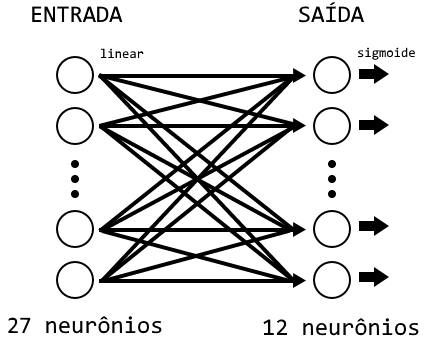
\includegraphics[scale=0.9]{img/GameNN.png}\\
		\vspace{0.5mm}
		\source{Elaborado pelo autor.}
		\label{fig:gameNN}
	\end{figure}
	
	A camada de entrada possui 27 neurônios,
	que recebem valores entre -1000 e 1000.
	Em sua função de ativação,
	seus valores são multiplicados linearmente por uma constante de 0,002,
	reduzindo o intervalo dos valores para -2 e 2.
	
	A camada de saída possui 12 neurônios,
	e na função de entrada é feito um somatório dos estímulos vindos da camada de entrada multiplicados por um peso.
	Na função de ativação é aplicada a função sigmoide \eqref{eq:sigmoid}
	produzindo saídas no intervalo de 0 a 1
	(ilustrada na Figura \ref{fig:activationFunctions},
	gráfico \textbf{d},
	página \pageref{fig:activationFunctions}).
	
	\begin{equation}
		S(t) = \frac{1}{1 + e^{-t}}
		\label{eq:sigmoid}
	\end{equation}
	
	\vspace{3mm}
	
	A explicação sobre o uso de 27 neurônios na entrada e 12 na saída
	pode ser encontrada nas Tabelas \ref{tab:nnInput} e \ref{tab:nnOutput}, na Seção \ref{ssec:duranteABatalha}.
	
	A implementação foi feita com o uso de dois vetores e uma matriz,
	sendo que os vetores representam os neurônios da camada de entrada e saída,
	e a matriz é a matriz de pesos da RNA.
	Após o preenchimento do vetor de entrada e a matriz de pesos,
	são feitos os cálculos explicados acima para obter-se o vetor de saída,
	que é o resultado.
	
	\FloatBarrier
	\section{Algoritmo Genético Implementado}
	% Ligação com a seção anterior
	Os passos do AG aqui descrito irá detalhar o que foi introduzido na seção \textit{\ref{ssec:processo}} Processo (do AG).
	A Tabela \ref{tab:agCycle} e Figura \ref{fig:gaflow},
	das páginas \pageref{tab:agCycle} e \pageref{fig:gaflow},
	resumem a seção.
	Desta forma, o foco aqui será em descrever os detalhes de implementação.
	Valores aqui apresentados foram escolhidos com base em pesquisas sobre Algoritmo Genético.
	
	% Tamanho da população
	A população do AG implementado é composta por 40 indivíduos,
	sendo o cromossomo do indivíduo uma matriz de valores reais.
	% População inicializada
	Os genes do cromossomo são inicializados com valores aleatórios entre -1,0 e 1,0.
	
	% Avaliação: cálculo do fitness
	Na avaliação,
	dois indivíduos são selecionados e seus cromossomos
	(que representam a matriz de pesos na RNA)
	são carregados na Rede Neural Artificial.
	Após a execução da RNA em cada comando do jogo,
	é dada uma nota (\textit{fitness}) sobre a influência que a RNA causou,
	sendo que esta nota pode ser
	positiva se o resultado foi bom,
	ou negativa caso o resultado tenha sido indesejável.
	Mais detalhes sobre os cálculos serão mostrados na próxima seção:
	\ref{sec:funcionamentoDoJogo} Funcionamento do jogo.
	
	% Seleção - roleta e montagem da nova população
	% Elitismo
	Após a avaliação de todos os indivíduos da população,
	inicia-se o processo de seleção.
	Nesta parte, cria-se a nova população ainda vazia,
	e o objetivo passa a ser preenchê-la até ficar com 40 indivíduos.
	Os primeiros 2 indivíduos que entram na nova população são resultado do Elitismo,
	que copia os 2 com melhor \textit{fitness} da população antiga sem nenhuma modificação.
	
	Para as 38 vagas restantes,
	repete-se o seguinte processo para preenchê-las:
	Primeiro, seleciona-se 2 indivíduos usando o método da Roleta.
	% Crossover (uniforme), taxa
	Após isto, é calculado na taxa de \textit{crossover}, de 90\%, se haverá \textit{crossover} ou não.
	Caso haja, é aplicado o \textit{crossover} uniforme para a geração dos cromossomos filhos,
	que são adicionados na nova população.
	Caso não haja, os indivíduos selecionados são copiados para a nova população.
	
	% Mutação (taxa)
	Na última etapa, a de mutação, a nova população já está preenchida com 40 indivíduos.
	Para cada gene dos 38 cromossomos criados na seleção e \textit{crossover},
	é calculada uma chance de 1,5\% de se ocorrer a mutação.
	Se for determinado que haverá uma mutação em um gene,
	haverá uma alteração de 0,3 unidades para mais ou para menos nele,
	escolhido aleatoriamente.
	
	Finalizada a mutação,
	a nova população se torna a população atual e retorna-se na Avaliação,
	repetindo o processo.
	
	\FloatBarrier
	\section{Funcionamento do jogo} \label{sec:funcionamentoDoJogo}
	Visto a descrição das variáveis do jogo na seção 4.1
	e a explicação da implementação da Rede Neural Artificial e Algoritmo Genético nas seções 4.2 e 4.3,
	será explicado aqui como cada uma destas partes foram juntadas umas nas outras para formarem o todo,
	%que é um jogo jogado por uma Inteligência Artificial capaz de aprender e mostrar bons resultados.
	que é o trabalho desenvolvido.
	
	\subsection{Preparação da batalha}
	% Abertura do jogo pela primeira vez
	Ao abrir o jogo pela primeira vez,
	% criação da população e salvando os dados num arquivo (é salvo junto com a informação de quem já foi avaliado ou não)
	o script do Algoritmo Genético cria uma população aleatória e a salva em um arquivo.
	% Caso tenha fechado o jogo e aberto de novo, as informaçõoes são carregadas de arquivo.
	Desta forma, caso o jogo seja fechado e aberto novamente,
	as informações da população são carregadas do arquivo.
	Neste arquivo são salvos o número que representa a geração atual
	e informações de cada indivíduo da população: os cromossomos, seu \textit{fitness} e se o cromossomo já foi avaliado.
	
	% Primeiros 2 tem seus cromossomos carregados na RNA, uma para cada time
	Após a população ter sido criada ou carregada,
	procura-se os dois primeiros indivíduos que ainda não foram avaliados.
	Ao encontrar, a informação de seus cromossomos é carregada na matriz de pesos de uma RNA.
	Nesta parte, cada RNA representará a inteligência de um time,
	que por sua vez "emula"{} um jogador real.
	
	\subsection{Durante a batalha} \label{ssec:duranteABatalha}
	% Inicia-se a batalha, procura-se o primeiro a receber turno
	Ao iniciar a batalha, cada time tem uma RNA que a representa e controla.
	% O que recebeu turno roda a RNA respectiva a seu time
	O personagem que receber o turno é o que poderá efetuar um comando,
	e neste momento o \textit{script} de RNA do seu time entra em ação 6 vezes,
	uma para cada diferente personagem ainda em batalha.
	
	% Explicar quais são os valores de entrada que estão sendo usadas na camada de entrada
	Em cada execução da RNA, são usadas como entrada alguns parâmetros do personagem que possuí o turno,
	e parâmetros do possível alvo.
	As informações usadas como entrada na RNA estão descritas na Tabela \ref{tab:nnInput}.
	
	\begin{table}[h]
		\caption{Valores de entrada na RNA}
		\centering
		\small
		\renewcommand{\arraystretch}{1.2} % Aumenta espaçamento vertical
		\begin{tabular}{c|c|c|c}
			\hline 
			\textbf{Atacante}			& \multicolumn{2}{c|}{\textbf{Possível alvo}}	& \textbf{Outros}		\\\hline
			ATK							& HP perdido		& Def. Física*		& Alvo é inimigo?*				\\ 
			MAG							& MP usado			& Def. Água*		& Alvo está defendendo?*		\\ 
			SPD							& ATK				& Def. Fogo*		& 								\\ 
			Elem. Hab. Fraca* (5)		& DEF				& Def. Terra*		& 								\\ 
			Elem. Hab. Forte* (5)		& MAG				& Def. Vento*		& 								\\ 
										& RES									& 								\\
										& SPD									& 								\\\hline
		\end{tabular}\\
		\vspace{3mm}
		\source{Elaborado pelo autor.}
		\label{tab:nnInput}
	\end{table}
	
	% Explicação em detalhes de cada entrada na RNA
	No total são 27 entradas,
	em que os que foram marcados com um (X), sendo X um número,
	significa que aquele atributo ainda foi quebrado em X neurônios diferentes.
	Ou seja, no caso das habilidades,
	é subdividido em 5 neurônios para que cada um simbolize um elemento.
	%Já nos itens disponíveis,
	%são usados 6 neurônios por causa da existência de 6 diferentes itens.
	
	Valores na Tabela \ref{tab:nnInput} que contém um * (asterisco) representa que eles tem valor binário.
	Foi implementado que caso o valor seja "falso"{}, "não"{} ou "fraco"{}, terá o valor de entrada de -1000.
	Por outro lado, se o valor for "verdadeiro"{}, "sim"{} ou "forte"{}. terá o valor de entrada de 1000.
	
	Os demais valores vem com intervalo de 0 a 1000,
	mas que são convertidos para um intervalo de -1000 a 1000,
	ficando no mesmo padrão que as outras entradas.
	Como já visto na seção 4.2,
	o intervalo de -1000 a 1000 é multiplicado por uma constante para se reduzir ao intervalo de -2 a 2.
	
	% Explicar que cada valor de saída siginifica um comando e a chance de usar ele
	Após inserir esses dados nos neurônios de entrada da RNA da equipe,
	é possível fazer os cálculos para obter seus dados de saída,
	composto por 12 neurônios.
	
	Como já explicado, as saídas tem valores entre 0 e 1.
	A saída do primeiro neurônio é a que calcula a probabilidade daquele personagem se tornar alvo.
	Quanto mais próximo de 1, maior a probabilidade,
	e quanto mais próximo de 0, menor.
	Os outros 11 neurônios representam, cada um, a probabilidade de utilizar um determinado comando naquele personagem, caso ele vire alvo.
	O papel de cada neurônio de saída está ilustrada na Tabela \ref{tab:nnOutput}.
	
	\begin{table}[h]
		\caption{Significado dos valores de saída da RNA}
		\centering
		\small
		\renewcommand{\arraystretch}{1.2} % Aumenta espaçamento vertical
		\begin{tabular}{c|c|c}
			\thickhline 
			\textbf{Alvo}				& \textbf{Atacar}						& \textbf{Defender}				\\\hline
			Prob. de virar alvo			& Prob. de atacar						& Prob. de defender				\\\thickhline
			\textbf{Habilidade}			& 					\multicolumn{2}{c}{\textbf{Usar item}}				\\\hline
			Prob. usar a fraca			& Prob. item dano físico				& Prob. item dano terra			\\ 
			Prob. usar a forte			& Prob. item dano água					& Prob. item dano vento			\\ 
			Prob. usar a cura			& Prob. item dano fogo					& Prob. item poção				\\\thickhline
		\end{tabular}\\
		\vspace{3mm}
		\source{Elaborado pelo autor.}
		\label{tab:nnOutput}
	\end{table}
	
	%Então, na verificação de um personagem,
	%tem-se a probabilidade dele se tornar alvo e as 11 probabilidades de comandos para utilizar nele.
	Para utilizar esses dados,
	foi criada uma estrutura que une "alvo"{} a "comando"{} em uma única probabilidade,
	se segue a fórmula \eqref{eq:targetCommand} a seguir:
	
	\begin{equation}
		\textrm{Probabilidade} = 1,5 \times \textrm{Prob. de virar alvo} + \textrm{Prob. comando}
		\label{eq:targetCommand}
	\end{equation}
	
	\vspace{3mm}
	
	Desta forma, cria-se 11 combinações de alvo + comando em um personagem.
	Repetindo este processo nos $N$ personagens ainda em batalha,
	obtêm-se $11 \times N$ combinações de alvo e comando no final.
	
	Com todos estes resultados em mãos,
	é feita uma ordenação decrescente.
	% Verificação se é viável efetuar o comando (item ou disponível)
	Neste momento,
	o jogo tenta executar a melhor combinação de alvo e comando.
	Caso falhe (por falta de item ou MP),
	tenta-se executar o próximo comando da lista.
	% Efetua-se o comando
	Repete-se as tentativas até que consiga executar algum comando com sucesso.
	
	% Feedback do comando para avaliação (fitness)
	Após o comando ser executado pelo personagem,
	existe a avaliação de sua escolha.
	A nota inicial é 0 (zero),
	e a primeira verificação que se faz é atacou aliado ou curou inimigo.
	Caso tenha feito isto,
	recebe um decréscimo de 100 em sua nota.
	Caso contrário,
	se tiver atacado um inimigo ou curado um aliado,
	recebe um acréscimo de 50 pontos na nota.
	
	Logo em seguida,
	recebe também uma nota referente ao quão bom foi o dano ou cura.
	Em caso de dano,
	a nota é a que está representada na fórmula \eqref{eq:damageGrade} a seguir.
	
	\begin{equation}
		\textrm{Nota} = \textrm{dano}^{1,5}
		\label{eq:damageGrade}
	\end{equation}
	
	\vspace{3mm}
	
	Se este dano foi feito num inimigo,
	soma-se esta nota na que já foi previamente calculada.
	Por outro lado,
	se o dano foi em um aliado,
	subtrai-se na nota que já tem.
	
	Algo similar acontece na cura,
	que usa a fórmula \eqref{eq:healGrade} a seguir.
	
	\begin{equation}
		\textrm{Nota} = \textrm{cura}^{1,4}
		\label{eq:healGrade}
	\end{equation}
	
	\vspace{3mm}
	
	Inversamente ao dano,
	esta nota é acrescida se for feita em aliado e decrescida se for feita em inimigo.
	
	As fórmulas de dano e cura foram escolhidas de forma empírica,
	sendo escolhida a potência para encorajar danos/curas mais altas.
	Foi dado um pouco mais de vantagem para danos,
	uma vez que o objetivo do jogo é derrotar o time inimigo.
	
	% Bônus no fitness por derrotar (mostrar fórmula)
	Como última etapa na escolha da nota do comando verifica-se se o alvo foi derrotado,
	se sim um bônus na nota será dada.
	O bônus é inicialmente de 10.000 (dez mil) pontos,
	e reduz-se em 1,5\% de seu valor atual em cada turno a partir do primeiro personagem que efetuar seu segundo comando na batalha.
	O gráfico dos valores do bônus de derrotar está ilustrado na Figura \ref{fig:defeatBonusGraph}.
	O principal motivo da existência deste bônus é encorajar a estratégia de derrotar rapidamente os adversários,
	%um de cada vez,
	dado que cada personagem a menos no time inimigo é um a menos para causar danos no time aliado.
	
	\begin{figure}[ht!]
		\centering
		\caption{Bônus de derrotar inimigo}
		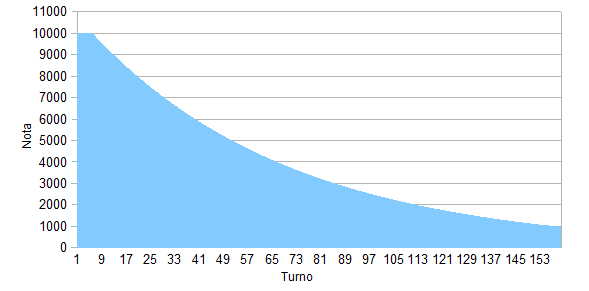
\includegraphics[scale=0.8]{img/DefeatBonusGraph.png}\\
		\vspace{0.5mm}
		\source{Elaborado pelo autor.}
		\label{fig:defeatBonusGraph}
	\end{figure}
	
	Todas estas notas que o personagem consegue e que são somadas são convertidas no \textit{fitness} do time (e da RNA).
	Uma batalha terá vários comandos executados pelo seu time,
	e quando a batalha acaba,
	todas as notas são somadas para obter o \textit{fitness} final da equipe.
	
	% Repete-se o processo até a batalha acabar
	Este processo de receber turno,
	rodar a Rede Neural Artificial,
	executar o comando e avaliá-la
	se repete até que uma das duas possíveis condições de parada sejam satisfeitas.
	% Condições de parada: time derrotado ou limite de turnos
	A primeira condição é um time completo derrotado.
	Neste caso, tem-se um vencedor, que é a equipe que ainda tem integrantes participando da batalha.
	A segunda condição é um limite de turnos,
	e o motivo dela é a existência de RNAs que enviam comandos de defender repetidamente aos personagens.
	Este limite turnos é verificado no valor do bônus ao derrotar:
	caso ele esteja com valor menor que 1.000 (mil),
	a batalha é encerrada com empate.
	
	\subsection{Após a batalha}
	% Finalizada a batalha, fitness das 2 populações são enviadas para o AG e salvas em arquivo
	Declarada o final da batalha,
	ter-se-á o valor de \textit{fitness} de ambas as equipes.
	Estes valores vão para o \textit{script} do Algoritmo Genético,
	que registra em sua estrutura o \textit{fitness} de cada um dos dois "indivíduos"{} e então salva no arquivo.
	
	% Carrega-se os 2 próximos e faz tudo novamente.
	Para continuar o treinamento da RNA,
	o \textit{script} do AG procura os dois próximos cromossomos que ainda não foram avaliados e carrega-os na RNA,
	repetindo todo o processo.
	% Após avaliar a população inteira, continuar no processo do AG para gerar a próxima geração, e repete tudo novamente
	Se todos os indivíduos da população já tiverem sido avaliados,
	o AG passa para a sua próxima etapa e cria a nova geração.

% DESENVOLVIMENTO - FIM

% CONCLUSÃO - INÍCIO
\FloatBarrier
\newpage % Coloca o conteúdo numa nova página
\chapter{RESULTADOS}

	Para o visual do jogo procurou-se deixá-lo o mais agradável possível,
	então foram usadas imagens disponibilizadas por usuários do site OpenGameArt\footnote{Link do site: \url{http://opengameart.org/}},
	e o resultado pode ser visto na Figura \ref{fig:gameScreenshot}.

	\begin{figure}[ht!]
		\centering
		\caption{\textit{Screenshot} do jogo}
		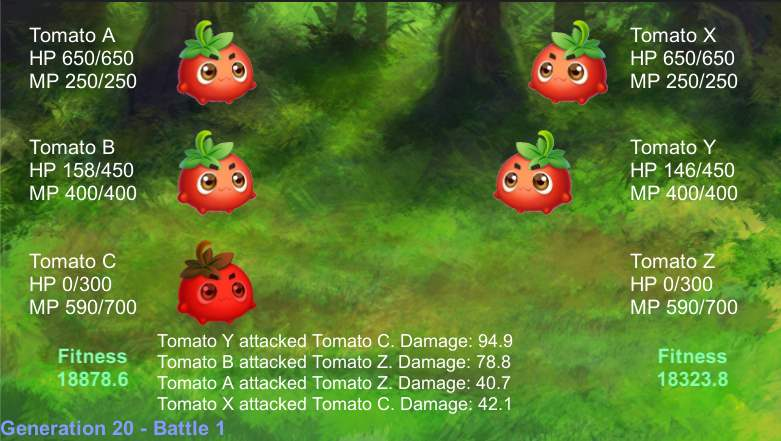
\includegraphics[scale=0.6]{img/GameScreenshot.jpg}\\
		\vspace{0.5mm}
		\source{Elaborado pelo autor.}
		\label{fig:gameScreenshot}
	\end{figure}

	Já a respeito da Inteligência Artificial,
	um treinamento de 50 gerações foi feito e os resultados estão ilustrados na Figura \ref{fig:fitnessResults}.
	
	\begin{figure}[ht!]
		\centering
		\caption{\textit{Fitness} durante 50 gerações}
		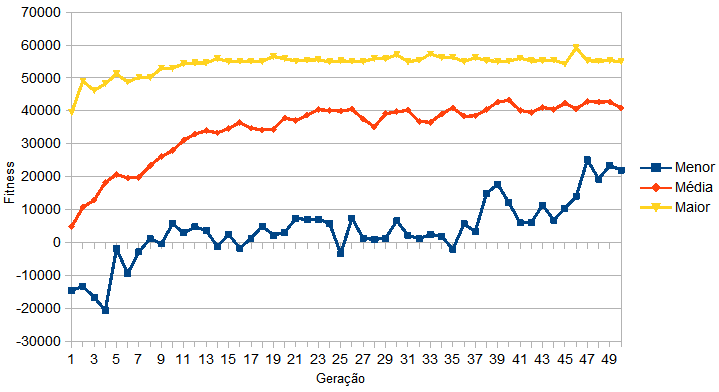
\includegraphics[scale=0.7]{img/AI-Result.png}\\
		\vspace{0.5mm}
		\source{Elaborado pelo autor.}
		\label{fig:fitnessResults}
	\end{figure}
	
	Percebeu-se que os personagens aprenderam a melhorar sua performance com sucesso,
	e com melhoras significativas nas primeiras gerações.
	Na primeira geração, a média de \textit{fitness} foi muito próxima a zero,
	o que mostra que quase metade das equipes tinha desempenho negativo.
	Este quadro muda completamente já na 10$^a$ geração,
	do qual a equipe de pior desempenho foi melhor que a média da primeira.
	
	É possível notar também que, coincidentemente,
	logo na primeira geração já houve uma equipe com alto desempenho.
	Esta equipe não só se manteve,
	 mas continuou melhorando lentamente.
	
	Por fim, o indicador que melhor mostrou a constante evolução da inteligência no jogo é a média do \textit{fitness},
	do qual é possível perceber um constante aumento,
	com apenas pequenas quedas pontuais.
	
% CONCLUSÃO - FIM
	\postextual
	\renewcommand{\bibname}{REFERÊNCIAS BIBLIOGRÁFICAS}
	\bibliography{referencias}

\end{document}
